% Options for packages loaded elsewhere
\PassOptionsToPackage{unicode}{hyperref}
\PassOptionsToPackage{hyphens}{url}
\PassOptionsToPackage{dvipsnames,svgnames,x11names}{xcolor}
%
\documentclass[
  bookmarksnumbered]{article}
\usepackage{amsmath,amssymb}
\usepackage{iftex}
\ifPDFTeX
  \usepackage[T1]{fontenc}
  \usepackage[utf8]{inputenc}
  \usepackage{textcomp} % provide euro and other symbols
\else % if luatex or xetex
  \usepackage{unicode-math} % this also loads fontspec
  \defaultfontfeatures{Scale=MatchLowercase}
  \defaultfontfeatures[\rmfamily]{Ligatures=TeX,Scale=1}
\fi
\usepackage{lmodern}
\ifPDFTeX\else
  % xetex/luatex font selection
\fi
% Use upquote if available, for straight quotes in verbatim environments
\IfFileExists{upquote.sty}{\usepackage{upquote}}{}
\IfFileExists{microtype.sty}{% use microtype if available
  \usepackage[]{microtype}
  \UseMicrotypeSet[protrusion]{basicmath} % disable protrusion for tt fonts
}{}
\makeatletter
\@ifundefined{KOMAClassName}{% if non-KOMA class
  \IfFileExists{parskip.sty}{%
    \usepackage{parskip}
  }{% else
    \setlength{\parindent}{0pt}
    \setlength{\parskip}{6pt plus 2pt minus 1pt}}
}{% if KOMA class
  \KOMAoptions{parskip=half}}
\makeatother
\usepackage{xcolor}
\usepackage[margin=2cm]{geometry}
\usepackage{color}
\usepackage{fancyvrb}
\newcommand{\VerbBar}{|}
\newcommand{\VERB}{\Verb[commandchars=\\\{\}]}
\DefineVerbatimEnvironment{Highlighting}{Verbatim}{commandchars=\\\{\}}
% Add ',fontsize=\small' for more characters per line
\usepackage{framed}
\definecolor{shadecolor}{RGB}{48,48,48}
\newenvironment{Shaded}{\begin{snugshade}}{\end{snugshade}}
\newcommand{\AlertTok}[1]{\textcolor[rgb]{1.00,0.81,0.69}{#1}}
\newcommand{\AnnotationTok}[1]{\textcolor[rgb]{0.50,0.62,0.50}{\textbf{#1}}}
\newcommand{\AttributeTok}[1]{\textcolor[rgb]{0.80,0.80,0.80}{#1}}
\newcommand{\BaseNTok}[1]{\textcolor[rgb]{0.86,0.64,0.64}{#1}}
\newcommand{\BuiltInTok}[1]{\textcolor[rgb]{0.80,0.80,0.80}{#1}}
\newcommand{\CharTok}[1]{\textcolor[rgb]{0.86,0.64,0.64}{#1}}
\newcommand{\CommentTok}[1]{\textcolor[rgb]{0.50,0.62,0.50}{#1}}
\newcommand{\CommentVarTok}[1]{\textcolor[rgb]{0.50,0.62,0.50}{\textbf{#1}}}
\newcommand{\ConstantTok}[1]{\textcolor[rgb]{0.86,0.64,0.64}{\textbf{#1}}}
\newcommand{\ControlFlowTok}[1]{\textcolor[rgb]{0.94,0.87,0.69}{#1}}
\newcommand{\DataTypeTok}[1]{\textcolor[rgb]{0.87,0.87,0.75}{#1}}
\newcommand{\DecValTok}[1]{\textcolor[rgb]{0.86,0.86,0.80}{#1}}
\newcommand{\DocumentationTok}[1]{\textcolor[rgb]{0.50,0.62,0.50}{#1}}
\newcommand{\ErrorTok}[1]{\textcolor[rgb]{0.76,0.75,0.62}{#1}}
\newcommand{\ExtensionTok}[1]{\textcolor[rgb]{0.80,0.80,0.80}{#1}}
\newcommand{\FloatTok}[1]{\textcolor[rgb]{0.75,0.75,0.82}{#1}}
\newcommand{\FunctionTok}[1]{\textcolor[rgb]{0.94,0.94,0.56}{#1}}
\newcommand{\ImportTok}[1]{\textcolor[rgb]{0.80,0.80,0.80}{#1}}
\newcommand{\InformationTok}[1]{\textcolor[rgb]{0.50,0.62,0.50}{\textbf{#1}}}
\newcommand{\KeywordTok}[1]{\textcolor[rgb]{0.94,0.87,0.69}{#1}}
\newcommand{\NormalTok}[1]{\textcolor[rgb]{0.80,0.80,0.80}{#1}}
\newcommand{\OperatorTok}[1]{\textcolor[rgb]{0.94,0.94,0.82}{#1}}
\newcommand{\OtherTok}[1]{\textcolor[rgb]{0.94,0.94,0.56}{#1}}
\newcommand{\PreprocessorTok}[1]{\textcolor[rgb]{1.00,0.81,0.69}{\textbf{#1}}}
\newcommand{\RegionMarkerTok}[1]{\textcolor[rgb]{0.80,0.80,0.80}{#1}}
\newcommand{\SpecialCharTok}[1]{\textcolor[rgb]{0.86,0.64,0.64}{#1}}
\newcommand{\SpecialStringTok}[1]{\textcolor[rgb]{0.80,0.58,0.58}{#1}}
\newcommand{\StringTok}[1]{\textcolor[rgb]{0.80,0.58,0.58}{#1}}
\newcommand{\VariableTok}[1]{\textcolor[rgb]{0.80,0.80,0.80}{#1}}
\newcommand{\VerbatimStringTok}[1]{\textcolor[rgb]{0.80,0.58,0.58}{#1}}
\newcommand{\WarningTok}[1]{\textcolor[rgb]{0.50,0.62,0.50}{\textbf{#1}}}
\usepackage{longtable,booktabs,array}
\usepackage{calc} % for calculating minipage widths
% Correct order of tables after \paragraph or \subparagraph
\usepackage{etoolbox}
\makeatletter
\patchcmd\longtable{\par}{\if@noskipsec\mbox{}\fi\par}{}{}
\makeatother
% Allow footnotes in longtable head/foot
\IfFileExists{footnotehyper.sty}{\usepackage{footnotehyper}}{\usepackage{footnote}}
\makesavenoteenv{longtable}
\usepackage{graphicx}
\makeatletter
\def\maxwidth{\ifdim\Gin@nat@width>\linewidth\linewidth\else\Gin@nat@width\fi}
\def\maxheight{\ifdim\Gin@nat@height>\textheight\textheight\else\Gin@nat@height\fi}
\makeatother
% Scale images if necessary, so that they will not overflow the page
% margins by default, and it is still possible to overwrite the defaults
% using explicit options in \includegraphics[width, height, ...]{}
\setkeys{Gin}{width=\maxwidth,height=\maxheight,keepaspectratio}
% Set default figure placement to htbp
\makeatletter
\def\fps@figure{htbp}
\makeatother
\setlength{\emergencystretch}{3em} % prevent overfull lines
\providecommand{\tightlist}{%
  \setlength{\itemsep}{0pt}\setlength{\parskip}{0pt}}
\setcounter{secnumdepth}{5}
\usepackage{caption} \usepackage{float} \floatplacement{figure}{H} \usepackage[utf8]{inputenc} \usepackage{fancyhdr} \pagestyle{fancy} \usepackage{hanging} \lhead{Vásquez-Amézquita et al.} \rhead{\textit{Exploring violence, resource access, and facial masculinity preferences}} \renewcommand{\abstractname}{Description} \usepackage[american]{babel} \usepackage{csquotes} \usepackage[style=apa,backend=biber]{biblatex} \DeclareLanguageMapping{american}{american-apa} \usepackage{hanging} \usepackage{amsthm,amssymb,amsfonts} \usepackage{tikz,lipsum,lmodern} \usepackage{multicol} \usepackage{orcidlink} \newcommand{\opensupplement}{\setcounter{table}{0} \renewcommand{\thetable}{S\arabic{table}} \setcounter{figure}{0} \renewcommand{\thefigure}{S\arabic{figure}}} \newcommand{\closesupplement}{\setcounter{table}{0} \renewcommand{\thetable}{\arabic{table}} \setcounter{figure}{0} \renewcommand{\thefigure}{\arabic{figure}}} \usepackage{multirow,booktabs,setspace} \DeclareCaptionLabelSeparator{point}{. } \captionsetup[table]{labelfont=bf, textfont=it, format=plain, labelsep=point, skip=5pt} \captionsetup[figure]{labelfont=bf, format=plain, justification=justified, singlelinecheck=false, labelsep=point, skip=5pt}
\usepackage{booktabs}
\usepackage{longtable}
\usepackage{array}
\usepackage{multirow}
\usepackage{wrapfig}
\usepackage{float}
\usepackage{colortbl}
\usepackage{pdflscape}
\usepackage{tabu}
\usepackage{threeparttable}
\usepackage{threeparttablex}
\usepackage[normalem]{ulem}
\usepackage{makecell}
\usepackage{xcolor}
\ifLuaTeX
  \usepackage{selnolig}  % disable illegal ligatures
\fi
\usepackage[]{biblatex}
\addbibresource{bib/Bibliography.bib}
\usepackage{bookmark}
\IfFileExists{xurl.sty}{\usepackage{xurl}}{} % add URL line breaks if available
\urlstyle{same}
\hypersetup{
  pdftitle={How do experiences of violence affect women's preferences for facial masculinity according to resource availability? An exploratory study using eye-tracking},
  pdfauthor={Milena Vásquez-Amézquita 1,3,; Andrés Castellanos-Chacón 2; Wendy Medina-Sarmiento1; Valentina Cepeda1; Marina Begoña Martínez-González 3; Juan David Leongómez 2},
  colorlinks=true,
  linkcolor={gray},
  filecolor={Maroon},
  citecolor={gray},
  urlcolor={blue},
  pdfcreator={LaTeX via pandoc}}

\title{How do experiences of violence affect women's preferences for facial masculinity according to resource availability? An exploratory study using eye-tracking}
\usepackage{etoolbox}
\makeatletter
\providecommand{\subtitle}[1]{% add subtitle to \maketitle
  \apptocmd{\@title}{\par {\large #1 \par}}{}{}
}
\makeatother
\subtitle{Code and analyses}
\author{Milena Vásquez-Amézquita \orcidlink{0000-0001-7317-8430}\textsuperscript{1,3,*} \and Andrés Castellanos-Chacón \orcidlink{0000-0003-1684-9319}\textsuperscript{2} \and Wendy Medina-Sarmiento\textsuperscript{1} \and Valentina Cepeda\textsuperscript{1} \and Marina Begoña Martínez-González \orcidlink{0000-0002-5840-6383}\textsuperscript{3} \and Juan David Leongómez \orcidlink{0000-0002-0092-6298}\textsuperscript{2}}
\date{17 September, 2024}

\begin{document}
\maketitle

\textsuperscript{1} Faculty of Psychology, Universidad El Bosque, Bogota, Colombia.\\
\textsuperscript{2} EvoCo: Human Behaviour and Evolution Lab, Faculty of Psychology, Universidad El Bosque, Bogota, Colombia\\
\textsuperscript{3} Faculty of Psychology, Universidad de la Costa, Barranquilla, Colombia.

\textsuperscript{*} Correspondence: \href{mailto:mvasquezam@unbosque.edu.co}{\href{mailto:mvasquezam@unbosque.edu.co}{\nolinkurl{mvasquezam@unbosque.edu.co}}}

\begin{center}\rule{0.5\linewidth}{0.5pt}\end{center}

\begin{center}
\textbf{Description}
\end{center}

\par
\begingroup
\leftskip3em
\rightskip\leftskip

This document contains all code, and step by step explanations for all analyses, figures and tables (including supplementary figures and tables) for:

\begin{hangparas}{.25in}{1}
Vásquez-Amézquita, M., Castellanos-Chacón, A., Medina-Sarmiento, W., Cepeda, V., Martínez-González, M. B., \& Leongómez, J. D.,  (in prep). \textit{How do experiences of violence affect women's preferences for facial masculinity according to resource availability? An exploratory study using eye-tracking.}
\end{hangparas}

Data available from the Open Science Framework (OSF): \url{https://doi.org/10.XXXXX/OSF.IO/XXXXX}. All analyses were planned by Milena Vásquez-Amézquita and Juan David Leongómez. This document and its underlying code were created in \texttt{R\ Markdown} by Juan David Leongómez using \LaTeX.

\begin{center}\rule{0.5\linewidth}{0.5pt}\end{center}

\par
\endgroup

{\hypersetup{hidelinks}
\setcounter{tocdepth}{6}
\tableofcontents
}
\opensupplement

\begin{center}\rule{0.5\linewidth}{0.5pt}\end{center}

\section{Preliminaries}\label{preliminaries}

\subsection{Load packages}\label{load-packages}

This file was created using \texttt{knitr} \autocite{knitrcit}, mostly using \texttt{tidyverse} \autocite{tidyversecit} syntax. As such, data wrangling was mainly done using packages such as \texttt{dplyr} \autocite{dplyrcit}, and most figures were created or modified using \texttt{ggplot2} \autocite{ggplotcit}. Tables were created using \texttt{knitr::kable} and \texttt{kableExtra} \autocite{kableExtracit}.

Linear mixed models were fitted using \texttt{lmerTest} \autocite{lmertestcit}, assumptions were performed using \texttt{performance} \autocite{ludecke2021}, contrasts and interactions were explored using \texttt{emmeans} \autocite{emmeanscit}.

Used packages also include \texttt{osfr} \autocite{osfrcit} to download and open data files directly from the Open Science Framework (\href{https://osf.io/}{OSF}), using the \texttt{osf\_retrieve\_file} and \texttt{osf\_download} functions.

All packages used in this file can be directly installed from the Comprehensive R Archive Network (\href{https://cran.r-project.org/}{CRAN}). For a complete list of packages used to create this file, and their versions, see section \ref{session}, at the end of the document.

\begin{Shaded}
\begin{Highlighting}[]
\FunctionTok{library}\NormalTok{(car)}
\FunctionTok{library}\NormalTok{(MASS)}
\FunctionTok{library}\NormalTok{(ggstats)}
\FunctionTok{library}\NormalTok{(tidyverse)}
\FunctionTok{library}\NormalTok{(ggpubr)}
\FunctionTok{library}\NormalTok{(readxl)}
\FunctionTok{library}\NormalTok{(lmerTest)}
\FunctionTok{library}\NormalTok{(emmeans)}
\FunctionTok{library}\NormalTok{(knitr)}
\FunctionTok{library}\NormalTok{(kableExtra)}
\FunctionTok{library}\NormalTok{(performance)}
\FunctionTok{library}\NormalTok{(GGally)}
\FunctionTok{library}\NormalTok{(scales)}
\FunctionTok{library}\NormalTok{(factoextra)}
\FunctionTok{library}\NormalTok{(FactoMineR)}
\FunctionTok{library}\NormalTok{(gtools)}
\FunctionTok{library}\NormalTok{(bbmle)}
\FunctionTok{library}\NormalTok{(effectsize)}
\end{Highlighting}
\end{Shaded}

\subsection{Custom functions}\label{custom-functions}

\subsubsection{\texorpdfstring{\texttt{pval.lev}}{pval.lev}}\label{pval.lev}

This function takes p-values and formats them in \LaTeX, highlighting significant results in bold.

\begin{Shaded}
\begin{Highlighting}[]
\CommentTok{\# Define a function \textquotesingle{}pval.lev\textquotesingle{} to format p{-}values based on specific thresholds.}
\NormalTok{pval.lev }\OtherTok{\textless{}{-}} \ControlFlowTok{function}\NormalTok{(pvals) \{}
  \CommentTok{\# If the p{-}value is less than 0.0001, return the string \textquotesingle{}\textbackslash{}textbf\{\textless{} 0.0001\}\textquotesingle{}.}
  \FunctionTok{ifelse}\NormalTok{(pvals }\SpecialCharTok{\textless{}} \FloatTok{0.0001}\NormalTok{,}
    \StringTok{"}\SpecialCharTok{\textbackslash{}\textbackslash{}}\StringTok{textbf\{\textless{} 0.0001\}"}\NormalTok{,}
    \CommentTok{\# If the p{-}value is less than 0.001, return the string \textquotesingle{}\textbackslash{}textbf\{\textless{} 0.001\}\textquotesingle{}.}
    \FunctionTok{ifelse}\NormalTok{(pvals }\SpecialCharTok{\textless{}} \FloatTok{0.001}\NormalTok{,}
      \StringTok{"}\SpecialCharTok{\textbackslash{}\textbackslash{}}\StringTok{textbf\{\textless{} 0.001\}"}\NormalTok{,}
      \CommentTok{\# If the p{-}value is less than 0.05, format it with bold text and round to 4}
      \CommentTok{\# decimal places.}
      \FunctionTok{ifelse}\NormalTok{(pvals }\SpecialCharTok{\textless{}} \FloatTok{0.05}\NormalTok{,}
        \FunctionTok{paste0}\NormalTok{(}\StringTok{"}\SpecialCharTok{\textbackslash{}\textbackslash{}}\StringTok{textbf\{"}\NormalTok{, }\FunctionTok{round}\NormalTok{(pvals, }\DecValTok{4}\NormalTok{), }\StringTok{"\}"}\NormalTok{),}
        \CommentTok{\# Otherwise, round the p{-}value to 2 decimal places.}
        \FunctionTok{round}\NormalTok{(pvals, }\DecValTok{2}\NormalTok{)}
\NormalTok{      )}
\NormalTok{    )}
\NormalTok{  )}
\NormalTok{\}}
\end{Highlighting}
\end{Shaded}

\subsubsection{\texorpdfstring{\texttt{corr.stars}}{corr.stars}}\label{corr.stars}

This function creates a correlation matrix, and displays significance (function \texttt{corr.stars} modified from \url{http://myowelt.blogspot.com/2008/04/beautiful-correlation-tables-in-r.html}).

\begin{Shaded}
\begin{Highlighting}[]
\NormalTok{corr.stars }\OtherTok{\textless{}{-}} \ControlFlowTok{function}\NormalTok{(x) \{}
  \CommentTok{\# Load the \textquotesingle{}Hmisc\textquotesingle{} package, which is required for the \textquotesingle{}rcorr\textquotesingle{} function.}
  \FunctionTok{require}\NormalTok{(Hmisc)}
  \CommentTok{\# Convert the input \textquotesingle{}x\textquotesingle{} to a matrix in case it is not already.}
\NormalTok{  x }\OtherTok{\textless{}{-}} \FunctionTok{as.matrix}\NormalTok{(x)}
  \CommentTok{\# Compute the correlation matrix (R) and p{-}values (p) using the \textquotesingle{}rcorr\textquotesingle{} function.}
\NormalTok{  R }\OtherTok{\textless{}{-}} \FunctionTok{rcorr}\NormalTok{(x)}\SpecialCharTok{$}\NormalTok{r }\CommentTok{\# Correlation matrix}
\NormalTok{  p }\OtherTok{\textless{}{-}} \FunctionTok{rcorr}\NormalTok{(x)}\SpecialCharTok{$}\NormalTok{P }\CommentTok{\# p{-}value matrix}
  \CommentTok{\# Define significance levels for the stars notation.}
  \CommentTok{\# *** for p \textless{} 0.001, ** for p \textless{} 0.01, * for p \textless{} 0.05, and † for p \textless{} 0.10.}
\NormalTok{  mystars }\OtherTok{\textless{}{-}} \FunctionTok{ifelse}\NormalTok{(p }\SpecialCharTok{\textless{}}\NormalTok{ .}\DecValTok{001}\NormalTok{,}
    \FunctionTok{paste0}\NormalTok{(}\StringTok{"}\SpecialCharTok{\textbackslash{}\textbackslash{}}\StringTok{textbf\{"}\NormalTok{, }\FunctionTok{round}\NormalTok{(R, }\DecValTok{2}\NormalTok{), }\StringTok{"***\}"}\NormalTok{),}
    \FunctionTok{ifelse}\NormalTok{(p }\SpecialCharTok{\textless{}}\NormalTok{ .}\DecValTok{01}\NormalTok{,}
      \FunctionTok{paste0}\NormalTok{(}\StringTok{"}\SpecialCharTok{\textbackslash{}\textbackslash{}}\StringTok{textbf\{"}\NormalTok{, }\FunctionTok{round}\NormalTok{(R, }\DecValTok{2}\NormalTok{), }\StringTok{"**\}"}\NormalTok{),}
      \FunctionTok{ifelse}\NormalTok{(p }\SpecialCharTok{\textless{}}\NormalTok{ .}\DecValTok{05}\NormalTok{,}
        \FunctionTok{paste0}\NormalTok{(}\StringTok{"}\SpecialCharTok{\textbackslash{}\textbackslash{}}\StringTok{textbf\{"}\NormalTok{, }\FunctionTok{round}\NormalTok{(R, }\DecValTok{2}\NormalTok{), }\StringTok{"*\}"}\NormalTok{),}
        \FunctionTok{ifelse}\NormalTok{(p }\SpecialCharTok{\textless{}}\NormalTok{ .}\DecValTok{10}\NormalTok{,}
          \FunctionTok{paste0}\NormalTok{(}\FunctionTok{round}\NormalTok{(R, }\DecValTok{2}\NormalTok{), }\StringTok{"$\^{}\{}\SpecialCharTok{\textbackslash{}\textbackslash{}}\StringTok{dagger\}$"}\NormalTok{),}
          \FunctionTok{format}\NormalTok{(}\FunctionTok{round}\NormalTok{(R, }\DecValTok{2}\NormalTok{), }\AttributeTok{nsmall =} \DecValTok{2}\NormalTok{)}
\NormalTok{        )}
\NormalTok{      )}
\NormalTok{    )}
\NormalTok{  )}
  \CommentTok{\# Build a new matrix \textquotesingle{}Rnew\textquotesingle{} that contains the correlations and their significance stars.}
\NormalTok{  Rnew }\OtherTok{\textless{}{-}} \FunctionTok{matrix}\NormalTok{(mystars,}
    \AttributeTok{ncol =} \FunctionTok{ncol}\NormalTok{(x)}
\NormalTok{  ) }\CommentTok{\# Ensure the new matrix has the same number of columns as \textquotesingle{}x\textquotesingle{}}
  \CommentTok{\# Add the correlation values without stars to the diagonal (self{-}correlations).}
  \FunctionTok{diag}\NormalTok{(Rnew) }\OtherTok{\textless{}{-}} \FunctionTok{paste}\NormalTok{(}\FunctionTok{diag}\NormalTok{(R), }\StringTok{" "}\NormalTok{,}
    \AttributeTok{sep =} \StringTok{""}
\NormalTok{  )}
  \CommentTok{\# Set row names and column names of the matrix \textquotesingle{}Rnew\textquotesingle{} to match those of the original matrix.}
  \FunctionTok{rownames}\NormalTok{(Rnew) }\OtherTok{\textless{}{-}} \FunctionTok{colnames}\NormalTok{(x)}
  \FunctionTok{colnames}\NormalTok{(Rnew) }\OtherTok{\textless{}{-}} \FunctionTok{paste}\NormalTok{(}\FunctionTok{colnames}\NormalTok{(x), }\StringTok{""}\NormalTok{, }\AttributeTok{sep =} \StringTok{""}\NormalTok{)}
  \CommentTok{\# Remove the upper triangle and the diagonal of the matrix to avoid duplication.}
\NormalTok{  Rnew }\OtherTok{\textless{}{-}} \FunctionTok{as.matrix}\NormalTok{(Rnew)}
\NormalTok{  Rnew[}\FunctionTok{upper.tri}\NormalTok{(Rnew, }\AttributeTok{diag =} \ConstantTok{TRUE}\NormalTok{)] }\OtherTok{\textless{}{-}} \StringTok{""}
  \CommentTok{\# Convert the matrix to a data frame for easier handling.}
\NormalTok{  Rnew }\OtherTok{\textless{}{-}} \FunctionTok{as.data.frame}\NormalTok{(Rnew)}
  \CommentTok{\# Remove the last column (empty column from the upper triangle) and return the result.}
\NormalTok{  Rnew }\OtherTok{\textless{}{-}} \FunctionTok{cbind}\NormalTok{(Rnew[}\DecValTok{1}\SpecialCharTok{:}\FunctionTok{length}\NormalTok{(Rnew) }\SpecialCharTok{{-}} \DecValTok{1}\NormalTok{])}
  \CommentTok{\# Return the final correlation matrix with significance stars.}
  \FunctionTok{return}\NormalTok{(Rnew)}
\NormalTok{\}}
\end{Highlighting}
\end{Shaded}

\subsection{Independent stimuli evaluation}\label{independent-stimuli-evaluation}

The sex typicality of all stimuli was manipulated to either enhance or reduce their sex-typical characteristics. Since all the stimuli were male faces, this involved masculinizing them to increase their typical sex characteristics and feminizing them to reduce those characteristics. Masculinized and feminized versions were independently rated for masculinity and estimated age by a panel of raters (not participants).

\begin{Shaded}
\begin{Highlighting}[]
\CommentTok{\# Load the \textquotesingle{}Evaluacion Manipulación Rostros.xlsx\textquotesingle{} Excel file into a data frame}
\NormalTok{ext\_val }\OtherTok{\textless{}{-}} \FunctionTok{read\_excel}\NormalTok{(}\StringTok{"Data/Evaluacion Manipulación Rostros.xlsx"}\NormalTok{)}
\end{Highlighting}
\end{Shaded}

\subsubsection{Masculinity ratings}\label{masculinity-ratings}

First, masculinity rating given to the masculinized and feminized versions of each stimuli were compared.

\begin{Shaded}
\begin{Highlighting}[]
\CommentTok{\# Select relevant columns and reshape the data into long format}
\NormalTok{masc\_dat }\OtherTok{\textless{}{-}}\NormalTok{ ext\_val }\SpecialCharTok{|\textgreater{}}
  \FunctionTok{select}\NormalTok{(}
\NormalTok{    ResponseId,}
    \FunctionTok{contains}\NormalTok{(}\StringTok{"M"}\NormalTok{, }\AttributeTok{ignore.case =} \ConstantTok{FALSE}\NormalTok{), }\CommentTok{\# Select columns that contain "M" (masculinity)}
    \SpecialCharTok{{-}}\NormalTok{Menstruacion}
\NormalTok{  ) }\SpecialCharTok{|\textgreater{}} \CommentTok{\# Exclude the \textquotesingle{}Menstruacion\textquotesingle{} (menstruation) column}
  \FunctionTok{pivot\_longer}\NormalTok{(}
    \AttributeTok{cols =} \FunctionTok{contains}\NormalTok{(}\StringTok{"M"}\NormalTok{, }\AttributeTok{ignore.case =} \ConstantTok{FALSE}\NormalTok{), }\CommentTok{\# Reshape to long format}
    \AttributeTok{names\_to =} \StringTok{"Stimulus"}\NormalTok{, }\CommentTok{\# Column with stimuli names}
    \AttributeTok{values\_to =} \StringTok{"Masculinity"}
\NormalTok{  ) }\SpecialCharTok{|\textgreater{}} \CommentTok{\# Column with masculinity ratings}
  \CommentTok{\# Add a column indicating sexual dimorphism based on stimulus name}
  \FunctionTok{mutate}\NormalTok{(}\AttributeTok{Sexual\_dimorphism =} \FunctionTok{ifelse}\NormalTok{(}\FunctionTok{grepl}\NormalTok{(}\StringTok{"f\_1"}\NormalTok{, Stimulus), }\StringTok{"Feminine"}\NormalTok{, }\StringTok{"Masculine"}\NormalTok{)) }\SpecialCharTok{|\textgreater{}}
  \CommentTok{\# Keep only the first 3 characters of the stimulus name}
  \FunctionTok{mutate}\NormalTok{(}\AttributeTok{Stimulus =} \FunctionTok{str\_sub}\NormalTok{(Stimulus, }\AttributeTok{end =} \DecValTok{3}\NormalTok{))}

\CommentTok{\# Group by stimulus and perform t{-}tests for masculinity ratings across}
\CommentTok{\# sexual dimorphism categories}
\NormalTok{t\_masc }\OtherTok{\textless{}{-}}\NormalTok{ masc\_dat }\SpecialCharTok{|\textgreater{}}
  \FunctionTok{group\_by}\NormalTok{(Stimulus) }\SpecialCharTok{|\textgreater{}}
  \FunctionTok{summarise}\NormalTok{(}
    \AttributeTok{t =} \FunctionTok{round}\NormalTok{(}\FunctionTok{t.test}\NormalTok{(Masculinity }\SpecialCharTok{\textasciitilde{}}\NormalTok{ Sexual\_dimorphism)}\SpecialCharTok{$}\NormalTok{statistic, }\DecValTok{2}\NormalTok{), }\CommentTok{\# Compute t values}
    \AttributeTok{p =} \FunctionTok{pval.lev}\NormalTok{(}\FunctionTok{t.test}\NormalTok{(Masculinity }\SpecialCharTok{\textasciitilde{}}\NormalTok{ Sexual\_dimorphism)}\SpecialCharTok{$}\NormalTok{p.value)}
\NormalTok{  ) }\SpecialCharTok{|\textgreater{}} \CommentTok{\# Compute p{-}value}
  \FunctionTok{ungroup}\NormalTok{()}

\CommentTok{\# Select the first 10 rows of the data \textquotesingle{}t\_masc\textquotesingle{}}
\NormalTok{t\_masc[}\DecValTok{1}\SpecialCharTok{:}\DecValTok{10}\NormalTok{, ] }\SpecialCharTok{|\textgreater{}}
  \CommentTok{\# Add the next 10 rows (11 to 20) as additional columns}
  \FunctionTok{cbind}\NormalTok{(t\_masc[}\DecValTok{11}\SpecialCharTok{:}\DecValTok{20}\NormalTok{, ]) }\SpecialCharTok{|\textgreater{}}
  \CommentTok{\# Add the next 10 rows (21 to 30) as additional columns}
  \FunctionTok{cbind}\NormalTok{(t\_masc[}\DecValTok{21}\SpecialCharTok{:}\DecValTok{30}\NormalTok{, ]) }\SpecialCharTok{|\textgreater{}}
  \CommentTok{\# Create a table using the \textquotesingle{}kable\textquotesingle{} function}
  \FunctionTok{kable}\NormalTok{(}
    \AttributeTok{booktabs =} \ConstantTok{TRUE}\NormalTok{, }\CommentTok{\# Use \textquotesingle{}booktabs\textquotesingle{} style for better{-}looking tables in LaTeX}
    \AttributeTok{digits =} \DecValTok{2}\NormalTok{, }\CommentTok{\# Round numerical values to 2 decimal places}
    \AttributeTok{align =} \StringTok{"c"}\NormalTok{, }\CommentTok{\# Center align all columns}
    \AttributeTok{linesep =} \StringTok{""}\NormalTok{, }\CommentTok{\# No lines between rows}
    \AttributeTok{caption =} \StringTok{"Difference in independent masculinity ratings given to each stimulus,}
\StringTok{               according to its sexual dimorphism manipulation (feminized {-} masculinized)"}\NormalTok{,}
    \CommentTok{\# Caption for the table}
    \AttributeTok{escape =} \ConstantTok{FALSE}\NormalTok{, }\CommentTok{\# Allow LaTeX commands in the table (e.g., italic or bold)}
    \AttributeTok{col.names =} \FunctionTok{rep}\NormalTok{(}\FunctionTok{c}\NormalTok{(}\StringTok{"Stimulus"}\NormalTok{, }\StringTok{"}\SpecialCharTok{\textbackslash{}\textbackslash{}}\StringTok{textit\{t\}"}\NormalTok{, }\StringTok{"}\SpecialCharTok{\textbackslash{}\textbackslash{}}\StringTok{textit\{p\}"}\NormalTok{), }\AttributeTok{times =} \DecValTok{3}\NormalTok{) }\CommentTok{\# Column names}
\NormalTok{  ) }\SpecialCharTok{|\textgreater{}}
  \CommentTok{\# Apply additional LaTeX styling to the table using \textquotesingle{}kable\_styling\textquotesingle{}}
  \FunctionTok{kable\_styling}\NormalTok{(}
    \AttributeTok{latex\_options =} \FunctionTok{c}\NormalTok{(}\StringTok{"HOLD\_position"}\NormalTok{, }\StringTok{"scale\_down"}\NormalTok{) }\CommentTok{\# Keep table position}
\NormalTok{  ) }\SpecialCharTok{|\textgreater{}}
  \CommentTok{\# Add vertical lines after the 3rd and 6th columns using \textquotesingle{}column\_spec\textquotesingle{}}
  \FunctionTok{column\_spec}\NormalTok{(}\FunctionTok{c}\NormalTok{(}\DecValTok{3}\NormalTok{, }\DecValTok{6}\NormalTok{), }\AttributeTok{border\_right =} \ConstantTok{TRUE}\NormalTok{) }\SpecialCharTok{|\textgreater{}}
  \CommentTok{\# Add a footnote with specific formatting}
  \FunctionTok{footnote}\NormalTok{(}
    \AttributeTok{general =} \StringTok{"Tests are Welch\textquotesingle{}s }\SpecialCharTok{\textbackslash{}\textbackslash{}\textbackslash{}\textbackslash{}}\StringTok{textit\{t\}{-}test. Significant results are in bold."}\NormalTok{,}
    \CommentTok{\# General footnote text with LaTeX formatting}
    \AttributeTok{threeparttable =} \ConstantTok{TRUE}\NormalTok{, }\CommentTok{\# Enable three{-}part table for better layout}
    \AttributeTok{footnote\_as\_chunk =} \ConstantTok{TRUE}\NormalTok{, }\CommentTok{\# Render footnote as a chunk}
    \AttributeTok{escape =} \ConstantTok{FALSE} \CommentTok{\# Allow LaTeX commands in the footnote}
\NormalTok{  )}
\end{Highlighting}
\end{Shaded}

\begin{table}[H]
\centering
\caption{\label{tab:unnamed-chunk-5}Difference in independent masculinity ratings given to each stimulus,
               according to its sexual dimorphism manipulation (feminized - masculinized)}
\centering
\resizebox{\ifdim\width>\linewidth\linewidth\else\width\fi}{!}{
\begin{threeparttable}
\begin{tabular}[t]{cc>{}c|cc>{}c|ccc}
\toprule
Stimulus & \textit{t} & \textit{p} & Stimulus & \textit{t} & \textit{p} & Stimulus & \textit{t} & \textit{p}\\
\midrule
A01 & -6.09 & \textbf{< 0.0001} & A11 & -6.98 & \textbf{< 0.0001} & A21 & -7.81 & \textbf{< 0.0001}\\
A02 & -9.05 & \textbf{< 0.0001} & A12 & -7.90 & \textbf{< 0.0001} & A22 & -10.53 & \textbf{< 0.0001}\\
A03 & -8.96 & \textbf{< 0.0001} & A13 & -10.32 & \textbf{< 0.0001} & A23 & -6.83 & \textbf{< 0.0001}\\
A04 & -8.04 & \textbf{< 0.0001} & A14 & -7.76 & \textbf{< 0.0001} & A24 & -6.61 & \textbf{< 0.0001}\\
A05 & -9.81 & \textbf{< 0.0001} & A15 & -10.33 & \textbf{< 0.0001} & A25 & -8.18 & \textbf{< 0.0001}\\
A06 & -7.45 & \textbf{< 0.0001} & A16 & -10.63 & \textbf{< 0.0001} & A26 & -8.60 & \textbf{< 0.0001}\\
A07 & -7.04 & \textbf{< 0.0001} & A17 & -7.76 & \textbf{< 0.0001} & A27 & -6.55 & \textbf{< 0.0001}\\
A08 & -9.05 & \textbf{< 0.0001} & A18 & -10.29 & \textbf{< 0.0001} & A28 & -7.79 & \textbf{< 0.0001}\\
A09 & -12.18 & \textbf{< 0.0001} & A19 & -8.27 & \textbf{< 0.0001} & A29 & -11.25 & \textbf{< 0.0001}\\
A10 & -6.53 & \textbf{< 0.0001} & A20 & -9.72 & \textbf{< 0.0001} & A30 & -11.47 & \textbf{< 0.0001}\\
\bottomrule
\end{tabular}
\begin{tablenotes}[para]
\item \textit{Note: } 
\item Tests are Welch's \textit{t}-test. Significant results are in bold.
\end{tablenotes}
\end{threeparttable}}
\end{table}

\subsubsection{Age ratings}\label{age-ratings}

Then, estimated age of stimuli was assessed.

\begin{Shaded}
\begin{Highlighting}[]
\CommentTok{\# Process age{-}related data: select relevant columns and reshape into long format}
\NormalTok{age\_dat }\OtherTok{\textless{}{-}}\NormalTok{ ext\_val }\SpecialCharTok{|\textgreater{}}
  \FunctionTok{select}\NormalTok{(}
\NormalTok{    ResponseId,}
    \FunctionTok{contains}\NormalTok{(}\StringTok{"E"}\NormalTok{, }\AttributeTok{ignore.case =} \ConstantTok{FALSE}\NormalTok{)}
\NormalTok{  ) }\SpecialCharTok{|\textgreater{}} \CommentTok{\# Select columns related to estimated age (E)}
  \FunctionTok{select}\NormalTok{(}\SpecialCharTok{{-}}\FunctionTok{c}\NormalTok{(}\DecValTok{2}\SpecialCharTok{:}\DecValTok{5}\NormalTok{)) }\SpecialCharTok{|\textgreater{}} \CommentTok{\# Exclude columns 2 to 5 (irrelevant for this analysis)}
  \FunctionTok{pivot\_longer}\NormalTok{(}
    \AttributeTok{cols =} \FunctionTok{contains}\NormalTok{(}\StringTok{"E"}\NormalTok{, }\AttributeTok{ignore.case =} \ConstantTok{FALSE}\NormalTok{), }\CommentTok{\# Reshape to long format}
    \AttributeTok{names\_to =} \StringTok{"Stimulus"}\NormalTok{, }\CommentTok{\# Column with stimuli names}
    \AttributeTok{values\_to =} \StringTok{"Age"}
\NormalTok{  ) }\SpecialCharTok{|\textgreater{}} \CommentTok{\# Column with age estimates}
  \CommentTok{\# Add sexual dimorphism category based on stimulus name}
  \FunctionTok{mutate}\NormalTok{(}\AttributeTok{Sexual\_dimorphism =} \FunctionTok{ifelse}\NormalTok{(}\FunctionTok{grepl}\NormalTok{(}\StringTok{"f\_1"}\NormalTok{, Stimulus), }\StringTok{"Feminine"}\NormalTok{, }\StringTok{"Masculine"}\NormalTok{)) }\SpecialCharTok{|\textgreater{}}
  \CommentTok{\# Keep only the first 3 characters of the stimulus name}
  \FunctionTok{mutate}\NormalTok{(}\AttributeTok{Stimulus =} \FunctionTok{str\_sub}\NormalTok{(Stimulus, }\AttributeTok{end =} \DecValTok{3}\NormalTok{))}

\CommentTok{\# Summarize age data: compute mean, standard deviation, minimum, and maximum age}
\NormalTok{sum\_age\_dat }\OtherTok{\textless{}{-}}\NormalTok{ age\_dat }\SpecialCharTok{|\textgreater{}}
  \FunctionTok{summarise}\NormalTok{(}
    \AttributeTok{Mean =} \FunctionTok{mean}\NormalTok{(Age, }\AttributeTok{na.rm =} \ConstantTok{TRUE}\NormalTok{), }\CommentTok{\# Mean age}
    \AttributeTok{SD =} \FunctionTok{sd}\NormalTok{(Age, }\AttributeTok{na.rm =} \ConstantTok{TRUE}\NormalTok{), }\CommentTok{\# Standard deviation of age}
    \AttributeTok{Min =} \FunctionTok{min}\NormalTok{(Age, }\AttributeTok{na.rm =} \ConstantTok{TRUE}\NormalTok{), }\CommentTok{\# Minimum age}
    \AttributeTok{Max =} \FunctionTok{max}\NormalTok{(Age, }\AttributeTok{na.rm =} \ConstantTok{TRUE}\NormalTok{)}
\NormalTok{  ) }\CommentTok{\# Maximum age}
\end{Highlighting}
\end{Shaded}

\paragraph{Histogram of perceived age}\label{histogram-of-perceived-age}

Distribution of the estimated ages.

\begin{Shaded}
\begin{Highlighting}[]
\CommentTok{\# Create a histogram of estimated age}
\FunctionTok{ggplot}\NormalTok{(age\_dat, }\FunctionTok{aes}\NormalTok{(}\AttributeTok{x =}\NormalTok{ Age)) }\SpecialCharTok{+}
  \FunctionTok{geom\_histogram}\NormalTok{(}\AttributeTok{bins =} \DecValTok{26}\NormalTok{, }\AttributeTok{fill =} \StringTok{"\#6D9EC1"}\NormalTok{, }\AttributeTok{color =} \StringTok{"black"}\NormalTok{) }\SpecialCharTok{+} \CommentTok{\# Plot histogram with 26 bins}
  \FunctionTok{labs}\NormalTok{(}
    \AttributeTok{x =} \StringTok{"Estimated Age"}\NormalTok{, }\CommentTok{\# X{-}axis label}
    \AttributeTok{y =} \StringTok{"Count"}
\NormalTok{  ) }\SpecialCharTok{+} \CommentTok{\# Y{-}axis label}
  \FunctionTok{scale\_x\_continuous}\NormalTok{(}\AttributeTok{breaks =} \FunctionTok{seq}\NormalTok{(}\DecValTok{15}\NormalTok{, }\DecValTok{40}\NormalTok{, }\DecValTok{5}\NormalTok{)) }\CommentTok{\# X{-}axis scale with breaks every 5 units}
\end{Highlighting}
\end{Shaded}

\begin{figure}
\centering
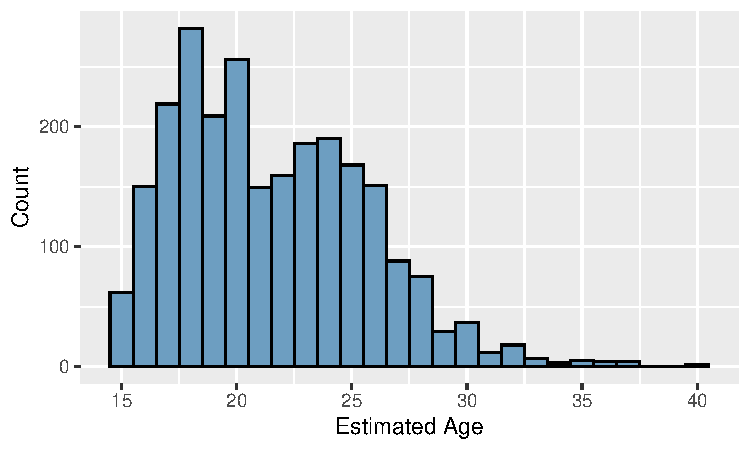
\includegraphics{Supplementary_material_files/figure-latex/estimated-age-hist-1.pdf}
\caption{\label{fig:estimated-age-hist}Histogram of estimated age of stimuli by an independent panel of raters. Age estimations were between 15 and 40 with a mean of 21.53 ± 4.11.}
\end{figure}

\subsection{Load and wrangle main experiment data}\label{load-and-wrangle-main-experiment-data}

\subsubsection{Individual databases (by data type/source)}\label{individual-databases-by-data-typesource}

\paragraph{Eye-tracking data}\label{eye-tracking-data}

\begin{Shaded}
\begin{Highlighting}[]
\CommentTok{\# Load the \textquotesingle{}CUC{-}UB\textquotesingle{} sheet from the \textquotesingle{}BD{-}ET{-}CUC{-}UB.xlsx\textquotesingle{} dataset}
\NormalTok{dat\_et }\OtherTok{\textless{}{-}} \FunctionTok{read\_excel}\NormalTok{(}\StringTok{"Data/BD{-}ET{-}CUC{-}UB.xlsx"}\NormalTok{,}
  \AttributeTok{sheet =} \StringTok{"CUC{-}UB"}
\NormalTok{) }\SpecialCharTok{|\textgreater{}}
  \CommentTok{\# Drop unused columns}
  \FunctionTok{select}\NormalTok{(}\SpecialCharTok{{-}}\FunctionTok{c}\NormalTok{(}
\NormalTok{    Participant, Condicion, TOI, Interval, Media\_respuesta, AOI,}
\NormalTok{    AOI\_Global, Respuesta, Number\_of\_mouse\_clicks...}\DecValTok{17}\NormalTok{,}
\NormalTok{    Time\_to\_first\_mouse\_click...}\DecValTok{18}\NormalTok{, AOI\_respuesta}
\NormalTok{  )) }\SpecialCharTok{|\textgreater{}}
  \CommentTok{\# Rename columns (to English)}
  \FunctionTok{rename}\NormalTok{(}
    \AttributeTok{ID =}\NormalTok{ Recording,}
    \AttributeTok{University =}\NormalTok{ UNIVERSIDAD,}
    \AttributeTok{Stimulus =}\NormalTok{ Media,}
    \AttributeTok{Condition =}\NormalTok{ Condición,}
    \AttributeTok{Relationship =}\NormalTok{ Contexto,}
    \AttributeTok{Sexual\_dimorphism =}\NormalTok{ Rostro,}
    \AttributeTok{TFD =}\NormalTok{ Total\_duration\_of\_whole\_fixations,}
    \AttributeTok{NF =}\NormalTok{ Number\_of\_whole\_fixations,}
    \AttributeTok{TFF =}\NormalTok{ Time\_to\_first\_whole\_fixation,}
    \AttributeTok{NMC =}\NormalTok{ Number\_of\_mouse\_clicks...}\DecValTok{21}\NormalTok{,}
    \AttributeTok{TFMC =}\NormalTok{ Time\_to\_first\_mouse\_click...}\DecValTok{22}\NormalTok{,}
    \AttributeTok{DFF =}\NormalTok{ Duration\_first\_fixation}
\NormalTok{  ) }\SpecialCharTok{|\textgreater{}}
  \CommentTok{\# Convert character columns to factors}
  \FunctionTok{mutate}\NormalTok{(}\FunctionTok{across}\NormalTok{(}\FunctionTok{where}\NormalTok{(is.character), as.factor)) }\SpecialCharTok{|\textgreater{}}
  \CommentTok{\# Recode factor levels to more meaningful English labels}
  \FunctionTok{mutate}\NormalTok{(}
    \AttributeTok{Condition =} \FunctionTok{fct\_recode}\NormalTok{(Condition,}
      \StringTok{"Low"} \OtherTok{=} \StringTok{"BAJA"}\NormalTok{,}
      \StringTok{"High"} \OtherTok{=} \StringTok{"ALTA"}
\NormalTok{    ),}
    \AttributeTok{Relationship =} \FunctionTok{fct\_recode}\NormalTok{(Relationship,}
      \StringTok{"Short term"} \OtherTok{=} \StringTok{"CP"}\NormalTok{,}
      \StringTok{"Long term"} \OtherTok{=} \StringTok{"LP"}
\NormalTok{    ),}
    \AttributeTok{Sexual\_dimorphism =} \FunctionTok{fct\_recode}\NormalTok{(Sexual\_dimorphism,}
      \StringTok{"Feminized"} \OtherTok{=} \StringTok{"Feminizado"}\NormalTok{,}
      \StringTok{"Masculinized"} \OtherTok{=} \StringTok{"Masculinizado"}
\NormalTok{    )}
\NormalTok{  ) }\SpecialCharTok{|\textgreater{}}
  \CommentTok{\# Modify \textquotesingle{}Stimulus\textquotesingle{} column to include \textquotesingle{}F\textquotesingle{} for Feminized and \textquotesingle{}M\textquotesingle{} for Masculinized}
  \FunctionTok{mutate}\NormalTok{(}
    \AttributeTok{Stimulus =} \FunctionTok{ifelse}\NormalTok{(Sexual\_dimorphism }\SpecialCharTok{==} \StringTok{"Feminized"}\NormalTok{,}
      \FunctionTok{paste0}\NormalTok{(}\FunctionTok{str\_sub}\NormalTok{(}\FunctionTok{str\_replace}\NormalTok{(Stimulus, }\StringTok{".* {-} "}\NormalTok{, }\StringTok{""}\NormalTok{), }\DecValTok{1}\NormalTok{, }\DecValTok{2}\NormalTok{), }\StringTok{"F"}\NormalTok{),}
      \FunctionTok{ifelse}\NormalTok{(Sexual\_dimorphism }\SpecialCharTok{==} \StringTok{"Masculinized"}\NormalTok{,}
        \FunctionTok{paste0}\NormalTok{(}\FunctionTok{str\_sub}\NormalTok{(}\FunctionTok{str\_replace}\NormalTok{(Stimulus, }\StringTok{".* {-} "}\NormalTok{, }\StringTok{""}\NormalTok{), }\DecValTok{1}\NormalTok{, }\DecValTok{2}\NormalTok{), }\StringTok{"M"}\NormalTok{),}
\NormalTok{        Stimulus}
\NormalTok{      )}
\NormalTok{    ),}
    \CommentTok{\# Create a new column \textquotesingle{}Choice\textquotesingle{} to indicate whether there was a mouse click}
    \AttributeTok{Choice =} \FunctionTok{ifelse}\NormalTok{(NMC }\SpecialCharTok{==} \DecValTok{0}\NormalTok{, }\StringTok{"No"}\NormalTok{, }\StringTok{"Yes"}\NormalTok{)}
\NormalTok{  )}
\end{Highlighting}
\end{Shaded}

\paragraph{Questionnaires}\label{questionnaires}

This was loaded without calculating total instrument scores (for now), to test internal consistency

\begin{Shaded}
\begin{Highlighting}[]
\NormalTok{quests }\OtherTok{\textless{}{-}} \FunctionTok{read\_excel}\NormalTok{(}\StringTok{"Data/Cuestionario Datos Sociodemográficos  (Disponibilidad) (respuestas) (1).xlsx"}\NormalTok{,}
  \AttributeTok{sheet =} \StringTok{"Respuestas de formulario 1"}
\NormalTok{) }\SpecialCharTok{|\textgreater{}}
  \CommentTok{\# Drop unnecessary columns (such as \textquotesingle{}Invitado\textquotesingle{}, \textquotesingle{}Servicios ayuda\textquotesingle{}, and \textquotesingle{}Correos cierre\textquotesingle{})}
  \FunctionTok{select}\NormalTok{(}\SpecialCharTok{{-}}\FunctionTok{c}\NormalTok{(Invitado, }\StringTok{\textasciigrave{}}\AttributeTok{Servicios ayuda}\StringTok{\textasciigrave{}}\NormalTok{, }\StringTok{\textasciigrave{}}\AttributeTok{Correos cierre}\StringTok{\textasciigrave{}}\NormalTok{)) }\SpecialCharTok{|\textgreater{}}
  \CommentTok{\# Rename columns for better readability}
  \FunctionTok{rename}\NormalTok{(}
    \AttributeTok{Date =}\NormalTok{ Fecha,}
    \AttributeTok{Age =}\NormalTok{ edad,}
    \AttributeTok{City =}\NormalTok{ Ciudad,}
    \AttributeTok{Education =}\NormalTok{ Escolaridad,}
    \AttributeTok{Ethnicity =}\NormalTok{ Etnia,}
    \AttributeTok{Gender =}\NormalTok{ Sexo,}
    \AttributeTok{Sex =}\NormalTok{ Genero,}
    \AttributeTok{Sexual\_orientation =}\NormalTok{ OS,}
    \AttributeTok{Relationship\_current =} \StringTok{"Pareja actual"}\NormalTok{,}
    \AttributeTok{Relationship\_duration =}\NormalTok{ DuracionR,}
    \AttributeTok{Relationship\_status =}\NormalTok{ EstadoR,}
    \AttributeTok{Partner\_sex =}\NormalTok{ SexoParejaActual,}
    \AttributeTok{Partner\_masculinity =}\NormalTok{ Masculinidad\_pareja,}
    \AttributeTok{Partner\_dominance =}\NormalTok{ Dominancia\_pareja,}
    \AttributeTok{Partner\_attractiveness =}\NormalTok{ Atractivo\_pareja,}
    \AttributeTok{Number\_of\_children =}\NormalTok{ NumHijos,}
    \AttributeTok{Hormonal\_contraception =} \StringTok{"Anticonceptivos hormonales"}\NormalTok{,}
    \AttributeTok{Contraceptive =}\NormalTok{ Cual\_anticonceptivo,}
    \AttributeTok{Last\_mentruation =} \StringTok{"Ultima menstruacion"}\NormalTok{,}
    \AttributeTok{Currently\_pregnant =} \StringTok{"Embarazo actual"}\NormalTok{,}
    \AttributeTok{Sexual\_abuse =} \StringTok{"Experiencia abuso sexual"}\NormalTok{,}
    \AttributeTok{Comments =}\NormalTok{ comentarios1,}
    \AttributeTok{Medical\_history =} \StringTok{"antecedentes medicos"}\NormalTok{,}
    \AttributeTok{SP\_happiness =} \StringTok{"AP felicidad"}\NormalTok{,}
    \AttributeTok{SP\_financial\_security =} \StringTok{"AP seguridad economica"}\NormalTok{,}
    \AttributeTok{SP\_money\_control =} \StringTok{"AP control dinero"}\NormalTok{,}
    \AttributeTok{SP\_attractiveness =} \StringTok{"AP atractivo"}\NormalTok{,}
    \AttributeTok{SP\_self\_confidence =} \StringTok{"AP autoconfianza"}\NormalTok{,}
    \AttributeTok{SP\_self\_esteem =} \StringTok{"AP autoestima"}\NormalTok{,}
    \AttributeTok{SP\_health =} \StringTok{"AP salud"}\NormalTok{,}
    \AttributeTok{Electricity =} \StringTok{"SB electricidad"}\NormalTok{,}
    \AttributeTok{Internet\_access =} \StringTok{"SB internet"}\NormalTok{,}
    \AttributeTok{TV =} \StringTok{"SB television"}\NormalTok{,}
    \AttributeTok{Internet\_use =} \StringTok{"Fr acceso internet"}\NormalTok{,}
    \AttributeTok{Hospital\_access =} \StringTok{"Acceso hospital"}\NormalTok{,}
    \AttributeTok{Freq\_illness =} \StringTok{"Fr enfermedades"}\NormalTok{,}
    \AttributeTok{Socioeconomic\_level =} \StringTok{"Estrato socioeconomico"}\NormalTok{,}
    \AttributeTok{Neighborhood =} \StringTok{"Barrio de residencia"}\NormalTok{,}
    \AttributeTok{Perceived\_neighborhood\_safety =} \StringTok{"Seguridad barrio"}\NormalTok{,}
    \AttributeTok{Perceived\_city\_safety =} \StringTok{"Seguridad ciudad"}\NormalTok{,}
    \AttributeTok{Perceived\_home\_safety =} \StringTok{"Seguridad hogar"}\NormalTok{,}
    \AttributeTok{Perceived\_country\_safety =} \StringTok{"Seguridad país"}\NormalTok{,}
    \AttributeTok{Freq\_robery =} \StringTok{"Fr de robos"}\NormalTok{,}
    \AttributeTok{Men\_perceived\_as\_danger\_to\_children =} \StringTok{"Hombres peligrosos hijos"}\NormalTok{,}
    \AttributeTok{Men\_perceived\_as\_danger\_to\_partner =} \StringTok{"Hombres peligrosos pareja"}\NormalTok{,}
    \AttributeTok{Partner\_physical\_violence =} \StringTok{"VP fisica"}\NormalTok{,}
    \AttributeTok{Freq\_partner\_physical\_violence =} \StringTok{"Fr VP fisica"}\NormalTok{,}
    \AttributeTok{Partner\_sexual\_violence =} \StringTok{"VP sexual"}\NormalTok{,}
    \AttributeTok{Freq\_partner\_sexual\_violence =} \StringTok{"Fr VP sexual"}\NormalTok{,}
    \AttributeTok{Partner\_infidelity =} \StringTok{"Infidelidad"}\NormalTok{,}
    \AttributeTok{Freq\_partner\_infidelity =} \StringTok{"Fr infidelidad"}\NormalTok{,}
    \AttributeTok{Victim\_of\_violence =} \StringTok{"Victima de alguna violencia"}\NormalTok{,}
    \AttributeTok{Violence\_type =} \StringTok{"Tipo violencia"}\NormalTok{,}
    \AttributeTok{Victim\_of\_gender\_violence =} \StringTok{"Victima violencia género"}\NormalTok{,}
    \AttributeTok{Victim\_of\_armed\_conflict =} \StringTok{"Victima conflicto armado"}\NormalTok{,}
    \AttributeTok{Control\_question\_1 =} \StringTok{"Sin leer"}\NormalTok{,}
    \AttributeTok{Control\_question\_2 =} \StringTok{"Broma"}
\NormalTok{  ) }\SpecialCharTok{|\textgreater{}}
  \CommentTok{\# Recode the factor levels of several categorical variables}
  \FunctionTok{mutate}\NormalTok{(}
    \AttributeTok{Education =} \FunctionTok{factor}\NormalTok{(Education, }\AttributeTok{levels =} \FunctionTok{c}\NormalTok{(}
      \StringTok{"Primaria"}\NormalTok{,}
      \StringTok{"Bachillerato"}\NormalTok{,}
      \StringTok{"Universitario"}\NormalTok{,}
      \StringTok{"Posgrado"}
\NormalTok{    )),}
    \AttributeTok{Sexual\_orientation =} \FunctionTok{factor}\NormalTok{(Sexual\_orientation,}
      \AttributeTok{levels =} \FunctionTok{c}\NormalTok{(}
        \StringTok{"Exclusivamente heterosexual"}\NormalTok{,}
        \StringTok{"Principalmente heterosexual, con contactos homosexuales esporádicos"}\NormalTok{,}
        \StringTok{"Predominantemente heterosexual, aunque con contactos homosexuales más que esporádicos"}\NormalTok{,}
        \StringTok{"Bisexual"}\NormalTok{,}
        \StringTok{"Pansexual"}\NormalTok{,}
        \StringTok{"Demisexual"}
\NormalTok{      )}
\NormalTok{    ),}
    \AttributeTok{Relationship\_status =} \FunctionTok{factor}\NormalTok{(Relationship\_status,}
      \AttributeTok{levels =} \FunctionTok{c}\NormalTok{(}
        \StringTok{"Soltero sin contactos sexuales en el último año"}\NormalTok{,}
        \StringTok{"Soltero con contactos sexuales en el último año"}\NormalTok{,}
        \StringTok{"Relación exclusiva o matrimonio {-} viven juntos"}\NormalTok{,}
        \StringTok{"Relación exclusiva {-} no viven juntos"}\NormalTok{,}
        \StringTok{"Relación no exclusiva {-} contactos sexuales con otras personas"}
\NormalTok{      )}
\NormalTok{    ),}
    \AttributeTok{Internet\_use =} \FunctionTok{factor}\NormalTok{(Internet\_use,}
      \AttributeTok{levels =} \FunctionTok{c}\NormalTok{(}\StringTok{"Cada día"}\NormalTok{, }\StringTok{"Cada mes"}\NormalTok{, }\StringTok{"Cada año"}\NormalTok{)}
\NormalTok{    ),}
    \AttributeTok{Socioeconomic\_level =} \FunctionTok{as.factor}\NormalTok{(Socioeconomic\_level)}
\NormalTok{  ) }\SpecialCharTok{|\textgreater{}}
  \CommentTok{\# Recode City variable to simplify geographical information}
  \FunctionTok{mutate}\NormalTok{(}\AttributeTok{City =} \FunctionTok{ifelse}\NormalTok{(City }\SpecialCharTok{\%in\%} \FunctionTok{c}\NormalTok{(}
    \StringTok{"Bogotá D.C."}\NormalTok{, }\StringTok{"Madrid, Cundinamarca"}\NormalTok{, }\StringTok{"Zipaquirá, Cundinamarca"}\NormalTok{,}
    \StringTok{"Zipaquirá"}\NormalTok{, }\StringTok{"Mosquera, cundinamarca"}\NormalTok{, }\StringTok{"Mosquera"}\NormalTok{,}
    \StringTok{"FUNZA, CUNDINAMARCA"}\NormalTok{, }\StringTok{"Madrid Cundinamarca"}\NormalTok{, }\StringTok{"Une{-} Cundinamarca"}
\NormalTok{  ),}
  \StringTok{"Bogota Region"}\NormalTok{,}
  \FunctionTok{ifelse}\NormalTok{(City }\SpecialCharTok{\%in\%} \FunctionTok{c}\NormalTok{(}
    \StringTok{"Soledad"}\NormalTok{, }\StringTok{"Barranquilla"}\NormalTok{, }\StringTok{"BARRANQUILLA"}\NormalTok{,}
    \StringTok{"Soledad, Atlantico"}\NormalTok{, }\StringTok{"Costa Atlantica"}\NormalTok{, }\StringTok{"Corozal"}
\NormalTok{  ),}
  \StringTok{"Atlantico Region"}\NormalTok{,}
  \StringTok{"Other"}
\NormalTok{  )}
\NormalTok{  )) }\SpecialCharTok{|\textgreater{}}
  \CommentTok{\# Recode several factors from Spanish to English for easier interpretation}
  \FunctionTok{mutate}\NormalTok{(}\AttributeTok{Education =} \FunctionTok{recode}\NormalTok{(Education,}
    \StringTok{"Primaria"} \OtherTok{=} \StringTok{"Primary school"}\NormalTok{,}
    \StringTok{"Bachillerato"} \OtherTok{=} \StringTok{"High school"}\NormalTok{,}
    \StringTok{"Universitario"} \OtherTok{=} \StringTok{"University"}\NormalTok{,}
    \StringTok{"Posgrado"} \OtherTok{=} \StringTok{"Postgraduate"}
\NormalTok{  )) }\SpecialCharTok{|\textgreater{}}
  \CommentTok{\# Additional recoding of variables}
  \FunctionTok{mutate}\NormalTok{(}\AttributeTok{Sexual\_orientation =} \FunctionTok{recode}\NormalTok{(Sexual\_orientation,}
    \StringTok{"Exclusivamente heterosexual"} \OtherTok{=}
      \StringTok{"Exclusively heterosexual"}\NormalTok{,}
    \StringTok{"Principalmente heterosexual, con contactos homosexuales esporádicos"} \OtherTok{=}
      \StringTok{"Predominantly heterosexual"}\NormalTok{,}
    \StringTok{"Predominantemente heterosexual, aunque con contactos homosexuales más que esporádicos"} \OtherTok{=}
      \StringTok{"Predominantly heterosexual, but more than incidentally homosexual"}\NormalTok{,}
    \StringTok{"Bisexual"} \OtherTok{=} \StringTok{"Bisexual"}\NormalTok{,}
    \StringTok{"Pansexual"} \OtherTok{=} \StringTok{"Pansexual"}\NormalTok{,}
    \StringTok{"Demisexual"} \OtherTok{=} \StringTok{"Demisexual"}
\NormalTok{  )) }\SpecialCharTok{|\textgreater{}}
  \FunctionTok{mutate}\NormalTok{(}\AttributeTok{Relationship\_status =} \FunctionTok{recode}\NormalTok{(Relationship\_status,}
    \StringTok{"Soltero sin contactos sexuales en el último año"} \OtherTok{=}
      \StringTok{"Single without sexual contacts"}\NormalTok{,}
    \StringTok{"Soltero con contactos sexuales en el último año"} \OtherTok{=}
      \StringTok{"Single with sexual contacts"}\NormalTok{,}
    \StringTok{"Relación exclusiva o matrimonio {-} viven juntos"} \OtherTok{=}
      \StringTok{"Exclusive relationship {-} cohabitating"}\NormalTok{,}
    \StringTok{"Relación exclusiva {-} no viven juntos"} \OtherTok{=}
      \StringTok{"Exclusive relationship {-} not cohabitating"}\NormalTok{,}
    \StringTok{"Relación no exclusiva {-} contactos sexuales con otras personas"} \OtherTok{=}
      \StringTok{"Non{-}exclusive relationship"}
\NormalTok{  )) }\SpecialCharTok{|\textgreater{}}
  \FunctionTok{mutate}\NormalTok{(}\AttributeTok{Internet\_use =} \FunctionTok{recode}\NormalTok{(Internet\_use,}
    \StringTok{"Cada día"} \OtherTok{=} \StringTok{"Daily"}\NormalTok{,}
    \StringTok{"Cada mes"} \OtherTok{=} \StringTok{"Monthly"}\NormalTok{,}
    \StringTok{"Cada año"} \OtherTok{=} \StringTok{"Yearly"}
\NormalTok{  )) }\SpecialCharTok{|\textgreater{}}
  \CommentTok{\# Recode several questions related to danger perceptions, replacing Spanish responses with}
  \CommentTok{\# numerical values.}
  \FunctionTok{mutate}\NormalTok{(}\FunctionTok{across}\NormalTok{(}
    \FunctionTok{starts\_with}\NormalTok{(}\StringTok{"Men\_perceived\_as\_danger\_to\_"}\NormalTok{),}
    \SpecialCharTok{\textasciitilde{}} \FunctionTok{recode}\NormalTok{(.,}
      \StringTok{"Completamente en desacuerdo"} \OtherTok{=} \DecValTok{1}\NormalTok{,}
      \StringTok{"Ligeramente en desacuerdo"} \OtherTok{=} \DecValTok{2}\NormalTok{,}
      \StringTok{"Ni de acuerdo ni en desacuerdo"} \OtherTok{=} \DecValTok{3}\NormalTok{,}
      \StringTok{"Ligeramente deacuerdo"} \OtherTok{=} \DecValTok{4}\NormalTok{,}
      \StringTok{"Completamente deacuerdo"} \OtherTok{=} \DecValTok{5}
\NormalTok{    )}
\NormalTok{  )) }\SpecialCharTok{|\textgreater{}}
  \CommentTok{\# Replace Spanish responses with corresponding English values}
  \FunctionTok{mutate}\NormalTok{(}\FunctionTok{across}\NormalTok{(}\FunctionTok{where}\NormalTok{(is.character), }\SpecialCharTok{\textasciitilde{}} \FunctionTok{replace}\NormalTok{(}
\NormalTok{    ., . }\SpecialCharTok{==}
      \StringTok{"Si"}\NormalTok{,}
    \StringTok{"Yes"}
\NormalTok{  ))) }\SpecialCharTok{|\textgreater{}}
  \FunctionTok{mutate}\NormalTok{(}\FunctionTok{across}\NormalTok{(}\FunctionTok{where}\NormalTok{(is.character), }\SpecialCharTok{\textasciitilde{}} \FunctionTok{replace}\NormalTok{(}
\NormalTok{    ., . }\SpecialCharTok{==}
      \StringTok{"Sí"}\NormalTok{,}
    \StringTok{"Yes"}
\NormalTok{  ))) }\SpecialCharTok{|\textgreater{}}
  \FunctionTok{mutate}\NormalTok{(}\FunctionTok{across}\NormalTok{(}\FunctionTok{where}\NormalTok{(is.character), }\SpecialCharTok{\textasciitilde{}} \FunctionTok{replace}\NormalTok{(}
\NormalTok{    ., . }\SpecialCharTok{==}
      \StringTok{"No quiero responder"}\NormalTok{,}
    \StringTok{"Prefer not to answer"}
\NormalTok{  ))) }\SpecialCharTok{|\textgreater{}}
  \FunctionTok{mutate}\NormalTok{(}\FunctionTok{across}\NormalTok{(}\FunctionTok{where}\NormalTok{(is.character), }\SpecialCharTok{\textasciitilde{}} \FunctionTok{replace}\NormalTok{(}
\NormalTok{    ., . }\SpecialCharTok{==}
      \StringTok{"Mujer"}\NormalTok{,}
    \StringTok{"Woman"}
\NormalTok{  ))) }\SpecialCharTok{|\textgreater{}}
  \FunctionTok{mutate}\NormalTok{(}\FunctionTok{across}\NormalTok{(}\FunctionTok{where}\NormalTok{(is.character), }\SpecialCharTok{\textasciitilde{}} \FunctionTok{replace}\NormalTok{(}
\NormalTok{    ., . }\SpecialCharTok{==}
      \StringTok{"Hombre"}\NormalTok{,}
    \StringTok{"Man"}
\NormalTok{  ))) }\SpecialCharTok{|\textgreater{}}
  \FunctionTok{mutate}\NormalTok{(}\FunctionTok{across}\NormalTok{(}\FunctionTok{where}\NormalTok{(is.character), }\SpecialCharTok{\textasciitilde{}} \FunctionTok{replace}\NormalTok{(}
\NormalTok{    ., . }\SpecialCharTok{==}
      \StringTok{"Femenino"}\NormalTok{,}
    \StringTok{"Female"}
\NormalTok{  ))) }\SpecialCharTok{|\textgreater{}}
  \FunctionTok{mutate}\NormalTok{(}\FunctionTok{across}\NormalTok{(}\FunctionTok{where}\NormalTok{(is.character), }\SpecialCharTok{\textasciitilde{}} \FunctionTok{replace}\NormalTok{(}
\NormalTok{    ., . }\SpecialCharTok{==}
      \StringTok{"Masculino"}\NormalTok{,}
    \StringTok{"Male"}
\NormalTok{  ))) }\SpecialCharTok{|\textgreater{}}
  \FunctionTok{mutate}\NormalTok{(}\FunctionTok{across}\NormalTok{(}\FunctionTok{where}\NormalTok{(is.character), }\SpecialCharTok{\textasciitilde{}} \FunctionTok{replace}\NormalTok{(}
\NormalTok{    ., . }\SpecialCharTok{==}
      \StringTok{"Sin pareja actual"}\NormalTok{,}
    \StringTok{"Single"}
\NormalTok{  ))) }\SpecialCharTok{|\textgreater{}}
  \FunctionTok{mutate}\NormalTok{(}\FunctionTok{across}\NormalTok{(}\FunctionTok{where}\NormalTok{(is.character), }\SpecialCharTok{\textasciitilde{}} \FunctionTok{replace}\NormalTok{(}
\NormalTok{    ., . }\SpecialCharTok{==}
      \StringTok{"Sí, una vez en la adultez"}\NormalTok{,}
    \StringTok{"Once as adult"}
\NormalTok{  ))) }\SpecialCharTok{|\textgreater{}}
  \FunctionTok{mutate}\NormalTok{(}\FunctionTok{across}\NormalTok{(}\FunctionTok{where}\NormalTok{(is.character), }\SpecialCharTok{\textasciitilde{}} \FunctionTok{replace}\NormalTok{(}
\NormalTok{    ., . }\SpecialCharTok{==}
      \StringTok{"Sí, tanto en la infancia como en la adultez"}\NormalTok{,}
    \StringTok{"Both as child and adult"}
\NormalTok{  ))) }\SpecialCharTok{|\textgreater{}}
  \FunctionTok{mutate}\NormalTok{(}\FunctionTok{across}\NormalTok{(}\FunctionTok{where}\NormalTok{(is.character), }\SpecialCharTok{\textasciitilde{}} \FunctionTok{replace}\NormalTok{(}
\NormalTok{    ., . }\SpecialCharTok{==}
      \StringTok{"Sí, más de una vez en mi infancia"}\NormalTok{,}
    \StringTok{"More than once as child"}
\NormalTok{  ))) }\SpecialCharTok{|\textgreater{}}
  \FunctionTok{mutate}\NormalTok{(}\FunctionTok{across}\NormalTok{(}\FunctionTok{where}\NormalTok{(is.character), }\SpecialCharTok{\textasciitilde{}} \FunctionTok{replace}\NormalTok{(}
\NormalTok{    ., . }\SpecialCharTok{==}
      \StringTok{"Sí, una vez e mi infancia"}\NormalTok{,}
    \StringTok{"Once as child"}
\NormalTok{  ))) }\SpecialCharTok{|\textgreater{}}
  \FunctionTok{mutate}\NormalTok{(}\FunctionTok{across}\NormalTok{(}\FunctionTok{where}\NormalTok{(is.character), }\SpecialCharTok{\textasciitilde{}} \FunctionTok{replace}\NormalTok{(}
\NormalTok{    ., . }\SpecialCharTok{==}
      \StringTok{"Afrocolombiano"}\NormalTok{,}
    \StringTok{"Afrocolombian"}
\NormalTok{  ))) }\SpecialCharTok{|\textgreater{}}
  \FunctionTok{mutate}\NormalTok{(}\FunctionTok{across}\NormalTok{(}\FunctionTok{where}\NormalTok{(is.character), }\SpecialCharTok{\textasciitilde{}} \FunctionTok{replace}\NormalTok{(}
\NormalTok{    ., . }\SpecialCharTok{==}
      \StringTok{"Desplazado conflicto armado"}\NormalTok{,}
    \StringTok{"Undetermined"}
\NormalTok{  ))) }\SpecialCharTok{|\textgreater{}}
  \FunctionTok{mutate}\NormalTok{(}\FunctionTok{across}\NormalTok{(}\FunctionTok{where}\NormalTok{(is.character), }\SpecialCharTok{\textasciitilde{}} \FunctionTok{replace}\NormalTok{(}
\NormalTok{    ., . }\SpecialCharTok{==}
      \StringTok{"Ninguna"}\NormalTok{,}
    \StringTok{"Undetermined"}
\NormalTok{  ))) }\SpecialCharTok{|\textgreater{}}
  \FunctionTok{mutate}\NormalTok{(}\FunctionTok{across}\NormalTok{(}\FunctionTok{where}\NormalTok{(is.character), }\SpecialCharTok{\textasciitilde{}} \FunctionTok{replace}\NormalTok{(}
\NormalTok{    ., . }\SpecialCharTok{==}
      \StringTok{"Comunidad negra"}\NormalTok{,}
    \StringTok{"Afrocolombian"}
\NormalTok{  ))) }\SpecialCharTok{|\textgreater{}}
  \FunctionTok{mutate}\NormalTok{(}\FunctionTok{across}\NormalTok{(}\FunctionTok{where}\NormalTok{(is.character), }\SpecialCharTok{\textasciitilde{}} \FunctionTok{replace}\NormalTok{(}
\NormalTok{    ., . }\SpecialCharTok{==}
      \StringTok{"Raizal del Archipiélago de San Andrés, Providencia y Santa Catalina"}\NormalTok{,}
    \StringTok{"Raizal"}
\NormalTok{  ))) }\SpecialCharTok{|\textgreater{}}
  \FunctionTok{mutate}\NormalTok{(}\FunctionTok{across}\NormalTok{(}\FunctionTok{where}\NormalTok{(is.character), }\SpecialCharTok{\textasciitilde{}} \FunctionTok{replace}\NormalTok{(}
\NormalTok{    ., . }\SpecialCharTok{==}
      \StringTok{"Patos"}\NormalTok{,}
    \StringTok{"Indigenous"}
\NormalTok{  ))) }\SpecialCharTok{|\textgreater{}}
  \FunctionTok{mutate}\NormalTok{(}\FunctionTok{across}\NormalTok{(}\FunctionTok{where}\NormalTok{(is.character), }\SpecialCharTok{\textasciitilde{}} \FunctionTok{replace}\NormalTok{(}
\NormalTok{    ., . }\SpecialCharTok{==}
      \StringTok{"Indígena"}\NormalTok{,}
    \StringTok{"Indigenous"}
\NormalTok{  ))) }\SpecialCharTok{|\textgreater{}}
  \FunctionTok{mutate}\NormalTok{(}\FunctionTok{across}\NormalTok{(}\FunctionTok{where}\NormalTok{(is.character), }\SpecialCharTok{\textasciitilde{}} \FunctionTok{replace}\NormalTok{(}
\NormalTok{    ., . }\SpecialCharTok{==}
      \StringTok{"No estoy segura"}\NormalTok{,}
    \StringTok{"Unsure"}
\NormalTok{  )))}
\end{Highlighting}
\end{Shaded}

\subparagraph{Principal component analysis (PCA)}\label{principal-component-analysis-pca}

To test whether it was possible to reduce the number of socio-ecological variables, we performed PCAs using the package FactoMineR \autocite{factominercit}, and plotted its results with function from the package factoextra \autocite{factoextracit}.

Socio-ecological factors PCA

\begin{Shaded}
\begin{Highlighting}[]
\CommentTok{\# Select relevant columns for PCA from the \textquotesingle{}quests\textquotesingle{} dataset}
\NormalTok{quests\_pca\_gen }\OtherTok{\textless{}{-}}\NormalTok{ quests }\SpecialCharTok{|\textgreater{}}
  \FunctionTok{select}\NormalTok{(}
\NormalTok{    ID, }\CommentTok{\# Unique identifier}
\NormalTok{    Men\_perceived\_as\_danger\_to\_partner,}
\NormalTok{    Men\_perceived\_as\_danger\_to\_children,}
\NormalTok{    Freq\_partner\_physical\_violence,}
\NormalTok{    Freq\_partner\_sexual\_violence,}
\NormalTok{    Freq\_partner\_infidelity,}
\NormalTok{    Perceived\_home\_safety}
\NormalTok{  ) }\SpecialCharTok{|\textgreater{}}
  \CommentTok{\# Rename columns: replace "Freq\_" with "Frequency of"}
  \FunctionTok{rename\_with}\NormalTok{(}\SpecialCharTok{\textasciitilde{}} \FunctionTok{str\_replace\_all}\NormalTok{(., }\StringTok{"Freq\_"}\NormalTok{, }\StringTok{"Frequency of"}\NormalTok{)) }\SpecialCharTok{|\textgreater{}}
  \CommentTok{\# Replace underscores with spaces in column names}
  \FunctionTok{rename\_with}\NormalTok{(}\SpecialCharTok{\textasciitilde{}} \FunctionTok{str\_replace\_all}\NormalTok{(., }\StringTok{"\_"}\NormalTok{, }\StringTok{" "}\NormalTok{)) }\SpecialCharTok{|\textgreater{}}
  \CommentTok{\# Capitalize the first letter of each column name}
  \FunctionTok{rename\_with}\NormalTok{(}\SpecialCharTok{\textasciitilde{}} \FunctionTok{str\_to\_sentence}\NormalTok{(.))}

\CommentTok{\# Perform PCA on the selected variables (excluding the ID column)}
\NormalTok{pca\_sef }\OtherTok{\textless{}{-}} \FunctionTok{PCA}\NormalTok{(quests\_pca\_gen[, }\SpecialCharTok{{-}}\DecValTok{1}\NormalTok{], }\AttributeTok{graph =} \ConstantTok{FALSE}\NormalTok{)}

\CommentTok{\# Display summary of the PCA results}
\NormalTok{pca\_sef}\SpecialCharTok{$}\NormalTok{var}\SpecialCharTok{$}\NormalTok{cor }\SpecialCharTok{|\textgreater{}}
  \CommentTok{\# Create a table using the \textquotesingle{}kable\textquotesingle{} function}
  \FunctionTok{kable}\NormalTok{(}
    \AttributeTok{booktabs =} \ConstantTok{TRUE}\NormalTok{, }\CommentTok{\# Use \textquotesingle{}booktabs\textquotesingle{} style for better{-}looking tables in LaTeX}
    \AttributeTok{digits =} \DecValTok{2}\NormalTok{, }\CommentTok{\# Round numerical values to 2 decimal places}
    \AttributeTok{align =} \StringTok{"c"}\NormalTok{, }\CommentTok{\# Center align all columns}
    \AttributeTok{linesep =} \StringTok{""}\NormalTok{, }\CommentTok{\# No lines between rows}
    \AttributeTok{caption =} \StringTok{"Correlation between variables and PCA dimensions"}\NormalTok{,}
    \CommentTok{\# Caption for the table}
    \AttributeTok{escape =} \ConstantTok{FALSE}\NormalTok{, }\CommentTok{\# Allow LaTeX commands in the table (e.g., italic or bold)}
\NormalTok{  ) }\SpecialCharTok{|\textgreater{}}
  \CommentTok{\# Apply additional LaTeX styling to the table using \textquotesingle{}kable\_styling\textquotesingle{}}
  \FunctionTok{kable\_styling}\NormalTok{(}
    \AttributeTok{latex\_options =} \FunctionTok{c}\NormalTok{(}\StringTok{"HOLD\_position"}\NormalTok{, }\StringTok{"scale\_down"}\NormalTok{) }\CommentTok{\# Keep table position}
\NormalTok{  )}
\end{Highlighting}
\end{Shaded}

\begin{table}[H]
\centering
\caption{\label{tab:pca-sef-tab}Correlation between variables and PCA dimensions}
\centering
\resizebox{\ifdim\width>\linewidth\linewidth\else\width\fi}{!}{
\begin{tabular}[t]{lccccc}
\toprule
  & Dim.1 & Dim.2 & Dim.3 & Dim.4 & Dim.5\\
\midrule
Men perceived as danger to partner & 0.89 & -0.27 & -0.03 & -0.13 & 0.01\\
Men perceived as danger to children & 0.89 & -0.25 & -0.04 & -0.11 & 0.03\\
Frequency ofpartner physical violence & 0.37 & 0.63 & 0.20 & 0.15 & -0.63\\
Frequency ofpartner sexual violence & 0.31 & 0.42 & -0.48 & 0.61 & 0.35\\
Frequency ofpartner infidelity & 0.19 & 0.59 & 0.54 & -0.32 & 0.48\\
Perceived home safety & 0.05 & -0.37 & 0.69 & 0.61 & 0.06\\
\bottomrule
\end{tabular}}
\end{table}

\textbf{Summary plot}

\begin{Shaded}
\begin{Highlighting}[]
\CommentTok{\# Arrange two plots side by side:}
\CommentTok{\# 1. A scree plot showing the explained variance for each principal component}
\CommentTok{\# 2. A plot showing the variable loadings on the principal components}
\FunctionTok{ggarrange}\NormalTok{(}
  \FunctionTok{fviz\_eig}\NormalTok{(pca\_sef, }\AttributeTok{addlabels =} \ConstantTok{TRUE}\NormalTok{, }\AttributeTok{barfill =} \StringTok{"\#00AFBB"}\NormalTok{) }\SpecialCharTok{+}
    \FunctionTok{labs}\NormalTok{(}
      \AttributeTok{title =} \StringTok{"PCA: Socio{-}ecological factors"}\NormalTok{, }\CommentTok{\# Title for the scree plot}
      \AttributeTok{subtitle =} \StringTok{"Scree plot"} \CommentTok{\# Subtitle for the scree plot}
\NormalTok{    ),}
  \FunctionTok{fviz\_pca\_var}\NormalTok{(pca\_sef,}
    \AttributeTok{col.var =} \StringTok{"\#00AFBB"}\NormalTok{, }\CommentTok{\# Color the variable loadings in teal}
    \AttributeTok{repel =} \ConstantTok{TRUE} \CommentTok{\# Avoid overlapping labels}
\NormalTok{  ) }\SpecialCharTok{+}
    \FunctionTok{labs}\NormalTok{(}
      \AttributeTok{title =} \ConstantTok{NULL}\NormalTok{, }\CommentTok{\# No title for the loading plot}
      \AttributeTok{subtitle =} \StringTok{"Loadings"} \CommentTok{\# Subtitle for the loading plot}
\NormalTok{    ),}
  \AttributeTok{labels =} \StringTok{"auto"}
\NormalTok{)}
\end{Highlighting}
\end{Shaded}

\begin{figure}
\centering
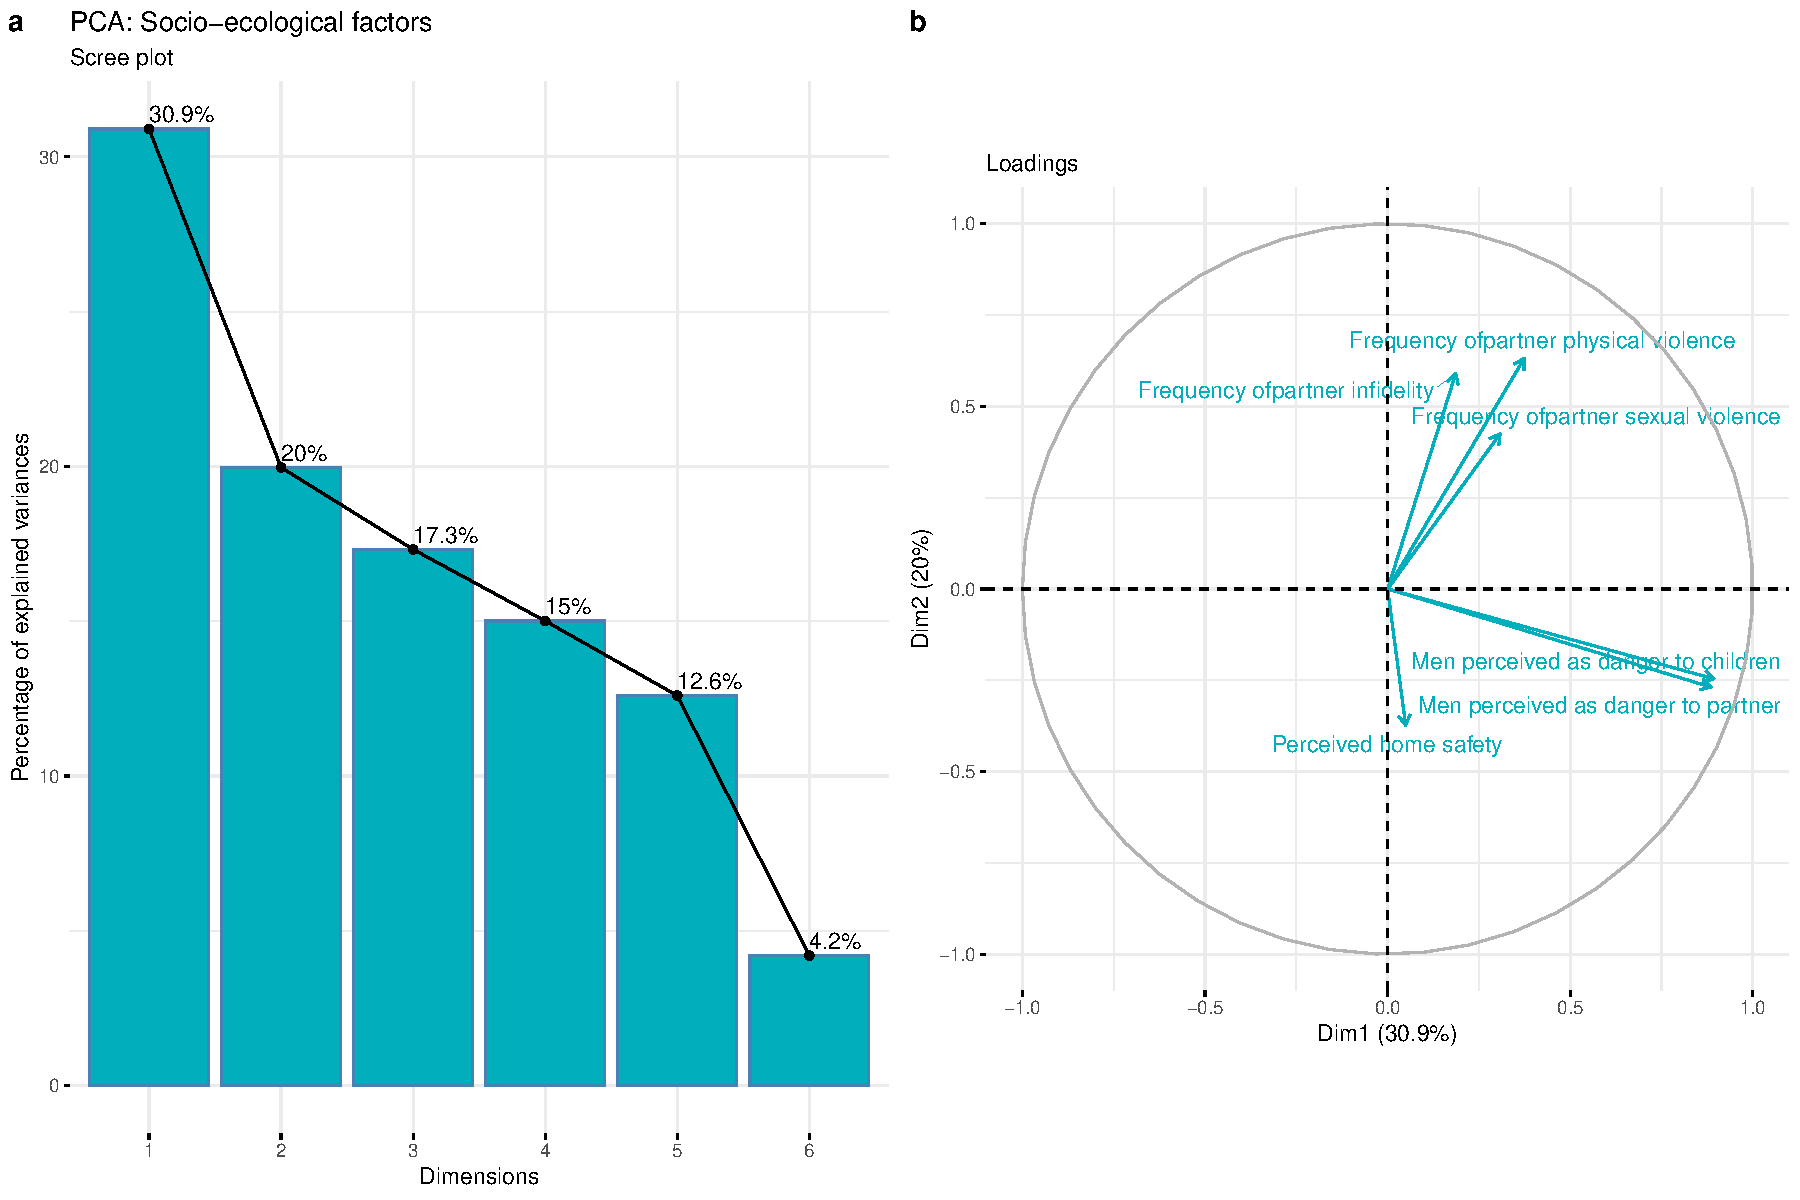
\includegraphics{Supplementary_material_files/figure-latex/pca-sef-plot-1.pdf}
\caption{\label{fig:pca-sef-plot}Summary of the PCA for all socio-ecological factors. \textbf{a.} Scree plot. \textbf{b.} Factor loadings.}
\end{figure}

When including all socio-ecological factors, the only variables that strongly correlate between them and with the PCA dimension (Table \ref{tab:pca-sef-plot}; Fig. \ref{fig:pca-sef-plot}), are the two variables that evaluate participant's perception of men as dangerous to children and to their partner.

Because of this, a new PCA was performed or only these two variables, to calculate a score of Men perceived as dangerous. All remaining socio-ecological variables were kept.

Men perceived as dangerous

\begin{Shaded}
\begin{Highlighting}[]
\CommentTok{\# Select relevant columns for PCA from the \textquotesingle{}quests\textquotesingle{} dataset}
\NormalTok{quests\_pca }\OtherTok{\textless{}{-}}\NormalTok{ quests }\SpecialCharTok{|\textgreater{}}
  \FunctionTok{select}\NormalTok{(}
\NormalTok{    ID,}
\NormalTok{    Men\_perceived\_as\_danger\_to\_partner,}
\NormalTok{    Men\_perceived\_as\_danger\_to\_children}
\NormalTok{  ) }\SpecialCharTok{|\textgreater{}}
  \CommentTok{\# Rename columns: remove "Men\_perceived\_as\_danger\_to\_"}
  \FunctionTok{rename\_with}\NormalTok{(}\SpecialCharTok{\textasciitilde{}} \FunctionTok{str\_remove\_all}\NormalTok{(., }\StringTok{"Men\_perceived\_as\_danger\_to\_"}\NormalTok{)) }\SpecialCharTok{|\textgreater{}}
  \CommentTok{\# Capitalize the first letter of each column name}
  \FunctionTok{rename\_with}\NormalTok{(}\SpecialCharTok{\textasciitilde{}} \FunctionTok{str\_to\_sentence}\NormalTok{(.))}


\CommentTok{\# Perform PCA on the selected variables (excluding the ID column)}
\NormalTok{pca\_mpd }\OtherTok{\textless{}{-}} \FunctionTok{PCA}\NormalTok{(quests\_pca[, }\SpecialCharTok{{-}}\DecValTok{1}\NormalTok{], }\AttributeTok{graph =} \ConstantTok{FALSE}\NormalTok{)}

\CommentTok{\# Calculate score for the men perceived as dangerous dimension}
\NormalTok{mpd\_scores }\OtherTok{\textless{}{-}} \FunctionTok{data.frame}\NormalTok{(pca\_mpd}\SpecialCharTok{$}\NormalTok{ind}\SpecialCharTok{$}\NormalTok{coord)}\SpecialCharTok{$}\NormalTok{Dim}\FloatTok{.1}

\CommentTok{\# Display summary of the PCA results}
\NormalTok{pca\_mpd}\SpecialCharTok{$}\NormalTok{var}\SpecialCharTok{$}\NormalTok{cor }\SpecialCharTok{|\textgreater{}}
  \CommentTok{\# Create a table using the \textquotesingle{}kable\textquotesingle{} function}
  \FunctionTok{kable}\NormalTok{(}
    \AttributeTok{booktabs =} \ConstantTok{TRUE}\NormalTok{, }\CommentTok{\# Use \textquotesingle{}booktabs\textquotesingle{} style for better{-}looking tables in LaTeX}
    \AttributeTok{digits =} \DecValTok{2}\NormalTok{, }\CommentTok{\# Round numerical values to 2 decimal places}
    \AttributeTok{align =} \StringTok{"c"}\NormalTok{, }\CommentTok{\# Center align all columns}
    \AttributeTok{linesep =} \StringTok{""}\NormalTok{, }\CommentTok{\# No lines between rows}
    \AttributeTok{caption =} \StringTok{"Correlation between variables and PCA dimensions"}\NormalTok{,}
    \CommentTok{\# Caption for the table}
    \AttributeTok{escape =} \ConstantTok{FALSE}\NormalTok{, }\CommentTok{\# Allow LaTeX commands in the table (e.g., italic or bold)}
\NormalTok{  ) }\SpecialCharTok{|\textgreater{}}
  \CommentTok{\# Apply additional LaTeX styling to the table using \textquotesingle{}kable\_styling\textquotesingle{}}
  \FunctionTok{kable\_styling}\NormalTok{(}
    \AttributeTok{latex\_options =} \FunctionTok{c}\NormalTok{(}\StringTok{"HOLD\_position"}\NormalTok{, }\StringTok{"scale\_down"}\NormalTok{) }\CommentTok{\# Keep table position}
\NormalTok{  )}
\end{Highlighting}
\end{Shaded}

\begin{table}[H]
\centering
\caption{\label{tab:unnamed-chunk-9}Correlation between variables and PCA dimensions}
\centering
\resizebox{\ifdim\width>\linewidth\linewidth\else\width\fi}{!}{
\begin{tabular}[t]{lcc}
\toprule
  & Dim.1 & Dim.2\\
\midrule
Partner & 0.93 & 0.36\\
Children & 0.93 & -0.36\\
\bottomrule
\end{tabular}}
\end{table}

\textbf{Summary plot}

In fact, the two variables related to men perceived as dangerous, could be reduced to a single dimension, that captured over 87\% of the variance.

\begin{Shaded}
\begin{Highlighting}[]
\CommentTok{\# Arrange two plots side by side:}
\CommentTok{\# 1. A scree plot showing the explained variance for each principal component}
\CommentTok{\# 2. A plot showing the variable loadings on the principal components}
\FunctionTok{ggarrange}\NormalTok{(}
  \FunctionTok{fviz\_eig}\NormalTok{(pca\_mpd, }\AttributeTok{addlabels =} \ConstantTok{TRUE}\NormalTok{, }\AttributeTok{barfill =} \StringTok{"\#00AFBB"}\NormalTok{) }\SpecialCharTok{+}
    \FunctionTok{labs}\NormalTok{(}
      \AttributeTok{title =} \StringTok{"PCA: Men perceived as danger to..."}\NormalTok{, }\CommentTok{\# Title for the scree plot}
      \AttributeTok{subtitle =} \StringTok{"Scree plot"} \CommentTok{\# Subtitle for the scree plot}
\NormalTok{    ),}
  \FunctionTok{fviz\_pca\_var}\NormalTok{(pca\_mpd,}
    \AttributeTok{col.var =} \StringTok{"\#00AFBB"}\NormalTok{, }\CommentTok{\# Color the variable loadings in teal}
    \AttributeTok{repel =} \ConstantTok{TRUE} \CommentTok{\# Avoid overlapping labels}
\NormalTok{  ) }\SpecialCharTok{+}
    \FunctionTok{labs}\NormalTok{(}
      \AttributeTok{title =} \ConstantTok{NULL}\NormalTok{, }\CommentTok{\# No title for the loading plot}
      \AttributeTok{subtitle =} \StringTok{"Loadings"} \CommentTok{\# Subtitle for the loading plot}
\NormalTok{    ),}
  \AttributeTok{labels =} \StringTok{"auto"}
\NormalTok{)}
\end{Highlighting}
\end{Shaded}

\begin{figure}
\centering
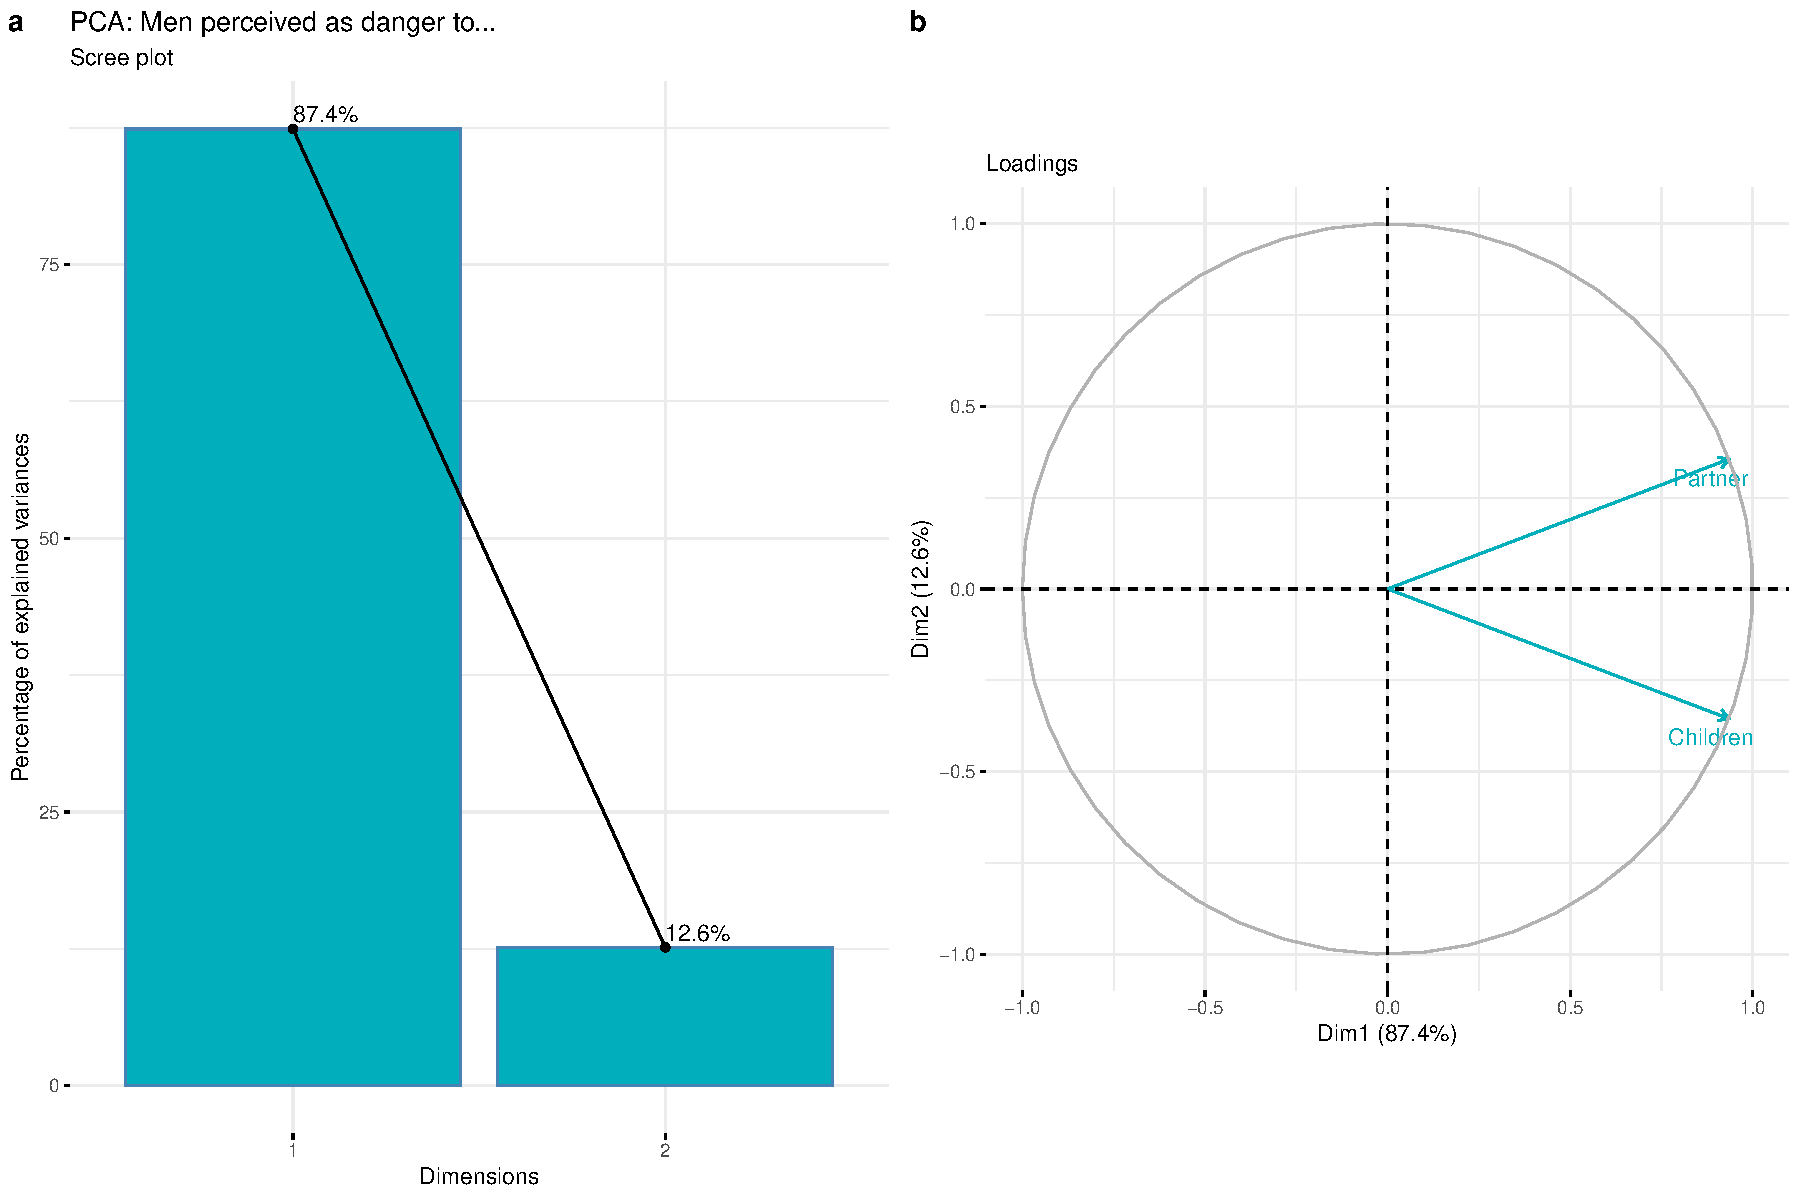
\includegraphics{Supplementary_material_files/figure-latex/pca-mpd-plot-1.pdf}
\caption{\label{fig:pca-mpd-plot}Summary of the PCA for factors related to men perceived as dangerous. \textbf{a.} Scree plot. \textbf{b.} Factor loadings.}
\end{figure}

\subparagraph{Clean questionnaire data}\label{clean-questionnaire-data}

Less columns, with total instrument scores

\begin{Shaded}
\begin{Highlighting}[]
\CommentTok{\# Clean and modify the \textquotesingle{}quests\textquotesingle{} dataset}
\NormalTok{quests\_clean }\OtherTok{\textless{}{-}}\NormalTok{ quests }\SpecialCharTok{|\textgreater{}}
  \CommentTok{\# Recode values in columns that start with "Escasez alimentaria"}
  \FunctionTok{mutate}\NormalTok{(}\FunctionTok{across}\NormalTok{(}
    \FunctionTok{starts\_with}\NormalTok{(}\StringTok{"Escasez alimentaria"}\NormalTok{),}
    \SpecialCharTok{\textasciitilde{}} \FunctionTok{recode}\NormalTok{(.,}
      \StringTok{"Nunca"} \OtherTok{=} \DecValTok{0}\NormalTok{, }\CommentTok{\# Recode "Nunca" to 0}
      \StringTok{"Rara vez/algunas veces"} \OtherTok{=} \DecValTok{1}\NormalTok{, }\CommentTok{\# Recode "Rara vez/algunas veces" to 1}
      \StringTok{"Casi siempre"} \OtherTok{=} \DecValTok{2} \CommentTok{\# Recode "Casi siempre" to 2}
\NormalTok{    )}
\NormalTok{  )) }\SpecialCharTok{|\textgreater{}}
  \CommentTok{\# Perform row{-}wise operations}
  \FunctionTok{rowwise}\NormalTok{() }\SpecialCharTok{|\textgreater{}}
  \CommentTok{\# Create new variables by summing up specific columns}
  \FunctionTok{mutate}\NormalTok{(}
    \CommentTok{\# Calculate Self{-}esteem score by summing relevant items (with reverse scoring)}
    \AttributeTok{Self\_esteem =} \FunctionTok{sum}\NormalTok{(}
\NormalTok{      autoestima\_I1, }\DecValTok{5} \SpecialCharTok{{-}}\NormalTok{ autoestima\_I2, autoestima\_I3, autoestima\_I4,}
\NormalTok{      autoestima\_I5, }\DecValTok{5} \SpecialCharTok{{-}}\NormalTok{ autoestima\_I6, autoestima\_I7, }\DecValTok{5} \SpecialCharTok{{-}}\NormalTok{ autoestima\_I8,}
      \DecValTok{5} \SpecialCharTok{{-}}\NormalTok{ autoestima\_I9, autoestima\_I10}
\NormalTok{    ),}
    \CommentTok{\# Calculate Self{-}perception score by summing columns that start with "SP\_"}
    \AttributeTok{Self\_perception =} \FunctionTok{sum}\NormalTok{(}\FunctionTok{across}\NormalTok{(}\FunctionTok{starts\_with}\NormalTok{(}\StringTok{"SP\_"}\NormalTok{))),}
    \CommentTok{\# Calculate Perceived safety by summing columns that end with "\_safety"}
    \AttributeTok{Perceived\_safety =} \FunctionTok{sum}\NormalTok{(}\FunctionTok{across}\NormalTok{(}\FunctionTok{ends\_with}\NormalTok{(}\StringTok{"\_safety"}\NormalTok{))),}
    \CommentTok{\# Calculate Food insecurity by summing columns that start with "Escasez alimentaria"}
    \AttributeTok{Food\_insecurity =} \FunctionTok{sum}\NormalTok{(}\FunctionTok{across}\NormalTok{(}\FunctionTok{starts\_with}\NormalTok{(}\StringTok{"Escasez alimentaria"}\NormalTok{)))}
\NormalTok{  ) }\SpecialCharTok{|\textgreater{}}
  \CommentTok{\# Remove columns that start with "autoestima\_"}
  \FunctionTok{select}\NormalTok{(}\SpecialCharTok{!}\FunctionTok{starts\_with}\NormalTok{(}\StringTok{"autoestima\_"}\NormalTok{)) }\SpecialCharTok{|\textgreater{}}
  \CommentTok{\# Convert character columns to factors}
  \FunctionTok{mutate}\NormalTok{(}\FunctionTok{across}\NormalTok{(}\FunctionTok{where}\NormalTok{(is.character), as.factor)) }\SpecialCharTok{|\textgreater{}}
  \CommentTok{\# Bind the column \textquotesingle{}Men\_perceived\_as\_dangerous\textquotesingle{} from \textquotesingle{}mpd\_scores\textquotesingle{} (PCA scores)}
  \FunctionTok{bind\_cols}\NormalTok{(}\AttributeTok{Men\_perceived\_as\_dangerous =}\NormalTok{ mpd\_scores)}
\end{Highlighting}
\end{Shaded}

\paragraph{Subjective evaluation of stimuli}\label{subjective-evaluation-of-stimuli}

\subparagraph{Wide format}\label{wide-format}

\begin{Shaded}
\begin{Highlighting}[]
\CommentTok{\# Load the subjective evaluation dataset, removing the last two columns (123 and 124)}
\NormalTok{eval }\OtherTok{\textless{}{-}} \FunctionTok{read\_excel}\NormalTok{(}\StringTok{"Data/Evaluación subjetiva rostros (Respuestas).xlsx"}\NormalTok{) }\SpecialCharTok{|\textgreater{}}
  \FunctionTok{select}\NormalTok{(}\SpecialCharTok{{-}}\FunctionTok{c}\NormalTok{(}\DecValTok{123}\SpecialCharTok{:}\DecValTok{124}\NormalTok{)) }\SpecialCharTok{|\textgreater{}}
  \CommentTok{\# Perform row{-}wise operations to compute new variables}
  \FunctionTok{rowwise}\NormalTok{() }\SpecialCharTok{|\textgreater{}}
  \CommentTok{\# Calculate the sum of masculinity and attractiveness ratings for both masculinized and}
  \CommentTok{\# feminized stimuli}
  \FunctionTok{mutate}\NormalTok{(}
    \AttributeTok{Masculinity\_masculinized =} \FunctionTok{sum}\NormalTok{(}\FunctionTok{across}\NormalTok{(}\FunctionTok{ends\_with}\NormalTok{(}\StringTok{"M Mas"}\NormalTok{))),}
    \AttributeTok{Masculinity\_feminized =} \FunctionTok{sum}\NormalTok{(}\FunctionTok{across}\NormalTok{(}\FunctionTok{ends\_with}\NormalTok{(}\StringTok{"F Mas"}\NormalTok{))),}
    \AttributeTok{Attractiveness\_masculinized =} \FunctionTok{sum}\NormalTok{(}\FunctionTok{across}\NormalTok{(}\FunctionTok{ends\_with}\NormalTok{(}\StringTok{"M Atr"}\NormalTok{))),}
    \AttributeTok{Attractiveness\_feminized =} \FunctionTok{sum}\NormalTok{(}\FunctionTok{across}\NormalTok{(}\FunctionTok{ends\_with}\NormalTok{(}\StringTok{"F Atr"}\NormalTok{)))}
\NormalTok{  ) }\SpecialCharTok{|\textgreater{}}
  \CommentTok{\# Rename columns for clarity}
  \FunctionTok{rename}\NormalTok{(}
    \AttributeTok{Date =} \StringTok{"Marca temporal"}\NormalTok{,}
    \AttributeTok{ID =} \StringTok{"Escribe tu código de participante"}
\NormalTok{  )}
\end{Highlighting}
\end{Shaded}

\subparagraph{Long format}\label{long-format}

\begin{Shaded}
\begin{Highlighting}[]
\CommentTok{\# Create a long format dataset by combining attractiveness and masculinity ratings}
\NormalTok{eval\_long }\OtherTok{\textless{}{-}} \FunctionTok{left\_join}\NormalTok{(}
  \CommentTok{\# First, select relevant columns and pivot the attractiveness ratings to long format}
\NormalTok{  eval }\SpecialCharTok{|\textgreater{}}
    \FunctionTok{select}\NormalTok{(}\SpecialCharTok{{-}}\FunctionTok{c}\NormalTok{(}\DecValTok{123}\SpecialCharTok{:}\DecValTok{126}\NormalTok{)) }\SpecialCharTok{|\textgreater{}} \CommentTok{\# Remove unnecessary columns}
    \FunctionTok{select}\NormalTok{(}\SpecialCharTok{!}\FunctionTok{ends\_with}\NormalTok{(}\StringTok{" Mas"}\NormalTok{)) }\SpecialCharTok{|\textgreater{}} \CommentTok{\# Exclude masculinity{-}related columns}
    \FunctionTok{pivot\_longer}\NormalTok{(}
      \AttributeTok{cols =} \FunctionTok{ends\_with}\NormalTok{(}\StringTok{"Atr"}\NormalTok{), }\CommentTok{\# Pivot attractiveness ratings to long format}
      \AttributeTok{names\_to =} \StringTok{"Stimulus"}\NormalTok{,}
      \AttributeTok{values\_to =} \StringTok{"Attractiveness"}
\NormalTok{    ) }\SpecialCharTok{|\textgreater{}}
    \FunctionTok{mutate}\NormalTok{(}\AttributeTok{Stimulus =} \FunctionTok{str\_remove\_all}\NormalTok{(Stimulus, }\StringTok{" Atr"}\NormalTok{)), }\CommentTok{\# Clean the Stimulus names}
  \CommentTok{\# Next, pivot the masculinity ratings to long format}
\NormalTok{  eval }\SpecialCharTok{|\textgreater{}}
    \FunctionTok{select}\NormalTok{(}\SpecialCharTok{{-}}\FunctionTok{c}\NormalTok{(}\DecValTok{123}\SpecialCharTok{:}\DecValTok{126}\NormalTok{)) }\SpecialCharTok{|\textgreater{}} \CommentTok{\# Remove unnecessary columns}
    \FunctionTok{select}\NormalTok{(}\SpecialCharTok{!}\FunctionTok{ends\_with}\NormalTok{(}\StringTok{" Atr"}\NormalTok{)) }\SpecialCharTok{|\textgreater{}} \CommentTok{\# Exclude attractiveness{-}related columns}
    \FunctionTok{pivot\_longer}\NormalTok{(}
      \AttributeTok{cols =} \FunctionTok{ends\_with}\NormalTok{(}\StringTok{"Mas"}\NormalTok{), }\CommentTok{\# Pivot masculinity ratings to long format}
      \AttributeTok{names\_to =} \StringTok{"Stimulus"}\NormalTok{,}
      \AttributeTok{values\_to =} \StringTok{"Masculinity"}
\NormalTok{    ) }\SpecialCharTok{|\textgreater{}}
    \FunctionTok{mutate}\NormalTok{(}\AttributeTok{Stimulus =} \FunctionTok{str\_remove\_all}\NormalTok{(Stimulus, }\StringTok{" Mas"}\NormalTok{)) }\CommentTok{\# Clean the Stimulus names}
\NormalTok{)}
\end{Highlighting}
\end{Shaded}

\paragraph{Resource availability}\label{resource-availability}

\begin{Shaded}
\begin{Highlighting}[]
\NormalTok{reg }\OtherTok{\textless{}{-}} \FunctionTok{rbind}\NormalTok{(}
  \FunctionTok{read\_excel}\NormalTok{(}\StringTok{"Data/3Registro Participantes Disponibilidad de Recursos{-}corregido.xlsx"}\NormalTok{,}
    \AttributeTok{sheet =} \StringTok{"UB"}
\NormalTok{  ) }\SpecialCharTok{|\textgreater{}}
    \FunctionTok{mutate}\NormalTok{(}\AttributeTok{University =} \StringTok{"UB"}\NormalTok{),}
  \FunctionTok{read\_excel}\NormalTok{(}\StringTok{"Data/3Registro Participantes Disponibilidad de Recursos{-}corregido.xlsx"}\NormalTok{,}
    \AttributeTok{sheet =} \StringTok{"CUC"}
\NormalTok{  ) }\SpecialCharTok{|\textgreater{}}
    \FunctionTok{mutate}\NormalTok{(}\AttributeTok{University =} \StringTok{"CUC"}\NormalTok{)}
\NormalTok{) }\SpecialCharTok{|\textgreater{}}
  \FunctionTok{select}\NormalTok{(}\SpecialCharTok{{-}}\FunctionTok{c}\NormalTok{(}
\NormalTok{    Grupo, }\StringTok{\textasciigrave{}}\AttributeTok{Entrega de kit}\StringTok{\textasciigrave{}}\NormalTok{, }\StringTok{\textasciigrave{}}\AttributeTok{Protocolo de bioseguridad}\StringTok{\textasciigrave{}}\NormalTok{, }\StringTok{\textasciigrave{}}\AttributeTok{Requisitos previos al registro}\StringTok{\textasciigrave{}}\NormalTok{, }
\NormalTok{    Consentimiento, }\StringTok{\textasciigrave{}}\AttributeTok{Código de evaluador}\StringTok{\textasciigrave{}}\SpecialCharTok{:}\StringTok{\textasciigrave{}}\AttributeTok{Código auxiliar que reclutó}\StringTok{\textasciigrave{}}
\NormalTok{  )) }\SpecialCharTok{|\textgreater{}}
  \FunctionTok{rename}\NormalTok{(}
    \AttributeTok{Date =} \StringTok{"Fecha de registro"}\NormalTok{,}
    \AttributeTok{ID =} \StringTok{"Codigo del Participante"}\NormalTok{,}
    \AttributeTok{Condition =} \StringTok{"Condicion"}\NormalTok{,}
    \AttributeTok{Calibration =} \StringTok{"Calibración"}\NormalTok{,}
    \AttributeTok{Gaze\_perc =} \StringTok{"\% Gaze"}\NormalTok{,}
    \AttributeTok{Condition\_happiness =} \StringTok{"Q Feliz"}\NormalTok{,}
    \AttributeTok{Condition\_physical\_safety =} \StringTok{"Q Segura físicamente"}\NormalTok{,}
    \AttributeTok{Condition\_healthy =} \StringTok{"Q Saludable"}\NormalTok{,}
    \AttributeTok{Condition\_economic\_security =} \StringTok{"Q Segura económicamente"}\NormalTok{,}
    \AttributeTok{Body\_temperature =} \StringTok{"Temperatura"}\NormalTok{,}
    \AttributeTok{Ovulating =} \StringTok{"Test de ovulación"}\NormalTok{,}
    \AttributeTok{Saliva\_pre =} \StringTok{"Recolección de saliva pre"}\NormalTok{,}
    \AttributeTok{Saliva\_pre\_time =} \StringTok{"Hora...18"}\NormalTok{,}
    \AttributeTok{Eye\_tracking =} \StringTok{"Rastreo Ocular"}\NormalTok{,}
    \AttributeTok{Subjective\_evaluation =} \StringTok{"Evaluación subjetiva"}\NormalTok{,}
    \AttributeTok{Sociodemographic\_questionnaire =} \StringTok{"Cuestionario sociodemográfico"}\NormalTok{,}
    \AttributeTok{Saliva\_post =} \StringTok{"Recolección de saliva post"}\NormalTok{,}
    \AttributeTok{Saliva\_post\_time =} \StringTok{"Hora...23"}\NormalTok{,}
    \AttributeTok{Notes =} \StringTok{"Observaciones"}
\NormalTok{  ) }\SpecialCharTok{|\textgreater{}}
  \FunctionTok{mutate}\NormalTok{(}
    \AttributeTok{Condition =} \FunctionTok{fct\_recode}\NormalTok{(Condition,}
      \StringTok{"Low"} \OtherTok{=} \StringTok{"Baja"}\NormalTok{,}
      \StringTok{"High"} \OtherTok{=} \StringTok{"Alta"}
\NormalTok{    ),}
    \AttributeTok{Calibration =} \FunctionTok{fct\_recode}\NormalTok{(Calibration,}
      \StringTok{"\textless{}=0.5"} \OtherTok{=} \StringTok{"\textless{}0.5 (menor a 0.5)"}\NormalTok{,}
      \StringTok{"\textgreater{}0.5"} \OtherTok{=} \StringTok{"\textgreater{}0.5 (mayor a 0.5)"}\NormalTok{,}
      \StringTok{"\textless{}=0.5"} \OtherTok{=} \StringTok{"0.5 (igual a 0.5)"}\NormalTok{,}
      \AttributeTok{NULL =} \StringTok{"Selecciona"}
\NormalTok{    ),}
    \AttributeTok{Ovulating =} \FunctionTok{fct\_recode}\NormalTok{(}\FunctionTok{as.factor}\NormalTok{(Ovulating),}
      \StringTok{"No"} \OtherTok{=} \StringTok{"0"}\NormalTok{,}
      \StringTok{"Yes"} \OtherTok{=} \StringTok{"1"}
\NormalTok{    )}
\NormalTok{  ) }\SpecialCharTok{|\textgreater{}}
  \FunctionTok{mutate\_all}\NormalTok{(}\SpecialCharTok{\textasciitilde{}} \FunctionTok{str\_replace\_all}\NormalTok{(., }\StringTok{"SI"}\NormalTok{, }\StringTok{"Yes"}\NormalTok{)) }\SpecialCharTok{|\textgreater{}}
  \FunctionTok{mutate\_all}\NormalTok{(}\SpecialCharTok{\textasciitilde{}} \FunctionTok{str\_replace\_all}\NormalTok{(., }\StringTok{"NO"}\NormalTok{, }\StringTok{"No"}\NormalTok{)) }\SpecialCharTok{|\textgreater{}}
  \FunctionTok{mutate\_all}\NormalTok{(}\SpecialCharTok{\textasciitilde{}} \FunctionTok{str\_replace\_all}\NormalTok{(., }\StringTok{"INCOMPLETO"}\NormalTok{, }\StringTok{"No"}\NormalTok{)) }\SpecialCharTok{|\textgreater{}}
  \FunctionTok{mutate\_all}\NormalTok{(}\SpecialCharTok{\textasciitilde{}} \FunctionTok{str\_replace\_all}\NormalTok{(., }\StringTok{"Recuperado"}\NormalTok{, }\StringTok{"Data recovered"}\NormalTok{)) }\SpecialCharTok{|\textgreater{}}
  \FunctionTok{mutate\_all}\NormalTok{(}\SpecialCharTok{\textasciitilde{}} \FunctionTok{str\_replace\_all}\NormalTok{(., }\StringTok{"RECUPERADO"}\NormalTok{, }\StringTok{"Data recovered"}\NormalTok{)) }\SpecialCharTok{|\textgreater{}}
  \FunctionTok{mutate\_all}\NormalTok{(}\SpecialCharTok{\textasciitilde{}} \FunctionTok{na\_if}\NormalTok{(., }\StringTok{"Selecciona"}\NormalTok{)) }\SpecialCharTok{|\textgreater{}}
  \FunctionTok{mutate\_all}\NormalTok{(}\SpecialCharTok{\textasciitilde{}} \FunctionTok{na\_if}\NormalTok{(., }\StringTok{"N/A"}\NormalTok{)) }\SpecialCharTok{|\textgreater{}}
  \FunctionTok{mutate}\NormalTok{(}\FunctionTok{across}\NormalTok{(}\FunctionTok{starts\_with}\NormalTok{(}\StringTok{"Condition\_"}\NormalTok{), as.numeric))}
\end{Highlighting}
\end{Shaded}

\subsubsection{Full, final database}\label{full-final-database}

\paragraph{Join data files}\label{join-data-files}

\begin{Shaded}
\begin{Highlighting}[]
\NormalTok{dat\_int }\OtherTok{\textless{}{-}}\NormalTok{ dat\_et }\SpecialCharTok{|\textgreater{}}
  \FunctionTok{left\_join}\NormalTok{(quests\_clean, }\AttributeTok{by =} \FunctionTok{c}\NormalTok{(}\StringTok{"ID"}\NormalTok{), }\AttributeTok{multiple =} \StringTok{"all"}\NormalTok{) }\SpecialCharTok{|\textgreater{}}
  \FunctionTok{left\_join}\NormalTok{(eval\_long, }\AttributeTok{by =} \FunctionTok{c}\NormalTok{(}\StringTok{"ID"}\NormalTok{, }\StringTok{"Stimulus"}\NormalTok{), }\AttributeTok{multiple =} \StringTok{"all"}\NormalTok{) }\SpecialCharTok{|\textgreater{}}
  \FunctionTok{left\_join}\NormalTok{(reg, }\AttributeTok{by =} \FunctionTok{c}\NormalTok{(}\StringTok{"ID"}\NormalTok{, }\StringTok{"University"}\NormalTok{, }\StringTok{"Condition"}\NormalTok{), }\AttributeTok{multiple =} \StringTok{"all"}\NormalTok{)}
\end{Highlighting}
\end{Shaded}

\paragraph{Filtered database}\label{filtered-database}

Filtered database to exclude participants who did responded the two control questions correctly, were ovulating, or did not report being exclusively heterosexual.

\begin{Shaded}
\begin{Highlighting}[]
\NormalTok{dat }\OtherTok{\textless{}{-}}\NormalTok{ dat\_int }\SpecialCharTok{|\textgreater{}}
  \CommentTok{\# Filter out rows where Control\_question\_1 and Control\_question\_2 are both "No",}
  \CommentTok{\# Ovulating is not "Yes", and Sexual\_orientation is "Exclusively heterosexual"}
  \FunctionTok{filter}\NormalTok{(Control\_question\_1 }\SpecialCharTok{==} \StringTok{"No"} \SpecialCharTok{\&}
\NormalTok{    Control\_question\_2 }\SpecialCharTok{==} \StringTok{"No"} \SpecialCharTok{\&}
\NormalTok{    Ovulating }\SpecialCharTok{!=} \StringTok{"Yes"} \SpecialCharTok{\&}
\NormalTok{    Sexual\_orientation }\SpecialCharTok{==} \StringTok{"Exclusively heterosexual"}\NormalTok{) }\SpecialCharTok{|\textgreater{}}
  \CommentTok{\# Remove all occurrences of the letter "F" from the Stimulus column}
  \CommentTok{\# (infomation already in the column Sexual\_dimorphism)}
  \FunctionTok{mutate}\NormalTok{(}\AttributeTok{Stimulus =} \FunctionTok{str\_remove\_all}\NormalTok{(Stimulus, }\StringTok{"F"}\NormalTok{)) }\SpecialCharTok{|\textgreater{}}
  \CommentTok{\# Remove all occurrences of the letter "M" from the Stimulus column}
  \CommentTok{\# (infomation already in the column Sexual\_dimorphism)}
  \FunctionTok{mutate}\NormalTok{(}\AttributeTok{Stimulus =} \FunctionTok{str\_remove\_all}\NormalTok{(Stimulus, }\StringTok{"M"}\NormalTok{)) }\SpecialCharTok{|\textgreater{}}
  \CommentTok{\# Ensure that the resulting data frame is ungrouped}
  \FunctionTok{ungroup}\NormalTok{()}
\end{Highlighting}
\end{Shaded}

After filtering the database and removing data who did not meet these criteria, from an initial sample size of 499 women, the final database contained data from 293 exclusively heterosexual participants, who were not ovulating.

\subsubsection{Final individual databases filtered to the final sample}\label{final-individual-databases-filtered-to-the-final-sample}

\paragraph{Resource availability (filtered)}\label{resource-availability-filtered}

\begin{Shaded}
\begin{Highlighting}[]
\NormalTok{reg\_fin }\OtherTok{\textless{}{-}}\NormalTok{ reg }\SpecialCharTok{|\textgreater{}}
  \FunctionTok{left\_join}\NormalTok{(quests\_clean, }\AttributeTok{by =} \FunctionTok{c}\NormalTok{(}\StringTok{"ID"}\NormalTok{)) }\SpecialCharTok{|\textgreater{}}
  \FunctionTok{filter}\NormalTok{(ID }\SpecialCharTok{\%in\%} \FunctionTok{unique}\NormalTok{(dat}\SpecialCharTok{$}\NormalTok{ID))}
\end{Highlighting}
\end{Shaded}

\paragraph{Questionnaires (filtered)}\label{questionnaires-filtered}

\begin{Shaded}
\begin{Highlighting}[]
\NormalTok{quests\_fin }\OtherTok{\textless{}{-}}\NormalTok{ quests\_clean }\SpecialCharTok{|\textgreater{}}
  \FunctionTok{filter}\NormalTok{(ID }\SpecialCharTok{\%in\%} \FunctionTok{unique}\NormalTok{(dat}\SpecialCharTok{$}\NormalTok{ID))}
\end{Highlighting}
\end{Shaded}

\section{Descriptives}\label{descriptives}

\subsection{Number and age of participants in each condition}\label{number-and-age-of-participants-in-each-condition}

\begin{Shaded}
\begin{Highlighting}[]
\NormalTok{dat }\SpecialCharTok{|\textgreater{}}
  \FunctionTok{group\_by}\NormalTok{(ID) }\SpecialCharTok{|\textgreater{}}
  \FunctionTok{summarise}\NormalTok{(}
    \AttributeTok{Age =} \FunctionTok{first}\NormalTok{(Age),}
    \AttributeTok{Condition =} \FunctionTok{first}\NormalTok{(Condition)}
\NormalTok{  ) }\SpecialCharTok{|\textgreater{}}
  \FunctionTok{ungroup}\NormalTok{() }\SpecialCharTok{|\textgreater{}}
  \FunctionTok{group\_by}\NormalTok{(Condition) }\SpecialCharTok{|\textgreater{}}
  \FunctionTok{summarise}\NormalTok{(}
    \AttributeTok{n =} \FunctionTok{n\_distinct}\NormalTok{(ID),}
    \AttributeTok{Mean =} \FunctionTok{mean}\NormalTok{(Age, }\AttributeTok{na.rm =} \ConstantTok{TRUE}\NormalTok{),}
    \AttributeTok{SD =} \FunctionTok{sd}\NormalTok{(Age, }\AttributeTok{na.rm =} \ConstantTok{TRUE}\NormalTok{),}
    \AttributeTok{Min =} \FunctionTok{min}\NormalTok{(Age, }\AttributeTok{na.rm =} \ConstantTok{TRUE}\NormalTok{),}
    \AttributeTok{Max =} \FunctionTok{max}\NormalTok{(Age, }\AttributeTok{na.rm =} \ConstantTok{TRUE}\NormalTok{)}
\NormalTok{  ) }\SpecialCharTok{|\textgreater{}}
  \FunctionTok{kable}\NormalTok{(}
    \AttributeTok{booktabs =} \ConstantTok{TRUE}\NormalTok{, }\CommentTok{\# Use \textquotesingle{}booktabs\textquotesingle{} style for better{-}looking tables in LaTeX}
    \AttributeTok{digits =} \DecValTok{2}\NormalTok{, }\CommentTok{\# Round numerical values to 2 decimal places}
    \AttributeTok{align =} \StringTok{"c"}\NormalTok{, }\CommentTok{\# Center align all columns}
    \AttributeTok{linesep =} \StringTok{""}\NormalTok{, }\CommentTok{\# No lines between rows}
    \AttributeTok{caption =} \StringTok{"Number and age of participants in each condition"}\NormalTok{,}
    \CommentTok{\# Caption for the table}
    \AttributeTok{escape =} \ConstantTok{FALSE}\NormalTok{, }\CommentTok{\# Allow LaTeX commands in the table (e.g., italic or bold)}
    \AttributeTok{col.names =} \FunctionTok{c}\NormalTok{(}
      \StringTok{"Condition"}\NormalTok{,}
      \StringTok{"}\SpecialCharTok{\textbackslash{}\textbackslash{}}\StringTok{textit\{n\}"}\NormalTok{,}
      \StringTok{"Mean"}\NormalTok{,}
      \StringTok{"SD"}\NormalTok{,}
      \StringTok{"Min."}\NormalTok{,}
      \StringTok{"Max."}
\NormalTok{    )}
\NormalTok{  ) }\SpecialCharTok{|\textgreater{}}
  \CommentTok{\# Apply additional LaTeX styling to the table using \textquotesingle{}kable\_styling\textquotesingle{}}
  \FunctionTok{kable\_styling}\NormalTok{(}
    \AttributeTok{latex\_options =} \FunctionTok{c}\NormalTok{(}\StringTok{"HOLD\_position"}\NormalTok{, }\StringTok{"scale\_down"}\NormalTok{) }\CommentTok{\# Keep table position}
\NormalTok{  )}
\end{Highlighting}
\end{Shaded}

\begin{table}[H]
\centering
\caption{\label{tab:unnamed-chunk-18}Number and age of participants in each condition}
\centering
\resizebox{\ifdim\width>\linewidth\linewidth\else\width\fi}{!}{
\begin{tabular}[t]{cccccc}
\toprule
Condition & \textit{n} & Mean & SD & Min. & Max.\\
\midrule
High & 165 & 21.41 & 2.25 & 18 & 27\\
Low & 128 & 21.50 & 2.25 & 18 & 25\\
\bottomrule
\end{tabular}}
\end{table}

\subsection{Select and wrangle data for descriptive plots}\label{select-and-wrangle-data-for-descriptive-plots}

\begin{Shaded}
\begin{Highlighting}[]
\CommentTok{\# Create desc\_quest, combining and transforming quests\_fin and reg}
\NormalTok{desc\_quest }\OtherTok{\textless{}{-}}
  \CommentTok{\# Join the quests\_fin and reg dataframes by ID}
\NormalTok{  quests\_fin }\SpecialCharTok{|\textgreater{}}
  \FunctionTok{left\_join}\NormalTok{(reg, }\AttributeTok{by =} \FunctionTok{c}\NormalTok{(}\StringTok{"ID"}\NormalTok{)) }\SpecialCharTok{|\textgreater{}}
  \CommentTok{\# Select only the desired columns}
  \FunctionTok{select}\NormalTok{(}
\NormalTok{    ID,}
\NormalTok{    Condition,}
\NormalTok{    Age,}
\NormalTok{    City,}
\NormalTok{    Education,}
\NormalTok{    Ethnicity,}
\NormalTok{    Sexual\_orientation,}
\NormalTok{    Relationship\_current,}
\NormalTok{    Relationship\_status}\SpecialCharTok{:}\NormalTok{Hormonal\_contraception,}
\NormalTok{    Sexual\_abuse,}
\NormalTok{    SP\_happiness}\SpecialCharTok{:}\NormalTok{Socioeconomic\_level,}
\NormalTok{    Perceived\_country\_safety}\SpecialCharTok{:}\NormalTok{Freq\_robery,}
\NormalTok{    Victim\_of\_violence,}
\NormalTok{    Victim\_of\_gender\_violence}\SpecialCharTok{:}\NormalTok{Victim\_of\_armed\_conflict,}
\NormalTok{    Self\_esteem}\SpecialCharTok{:}\NormalTok{Men\_perceived\_as\_dangerous,}
\NormalTok{    Freq\_partner\_physical\_violence,}
\NormalTok{    Freq\_partner\_infidelity,}
\NormalTok{    Partner\_physical\_violence,}
\NormalTok{    Partner\_sexual\_violence,}
\NormalTok{    Freq\_partner\_sexual\_violence,}
    \CommentTok{\# Food security variables (transformed later)}
    \StringTok{"Escasez alimentaria1"}\SpecialCharTok{:}\StringTok{"Escasez alimentaria5"}
\NormalTok{  ) }\SpecialCharTok{|\textgreater{}}
  \CommentTok{\# Transform all \textquotesingle{}Escasez alimentaria\textquotesingle{} (food scarcity) columns into categorical variables with }
  \CommentTok{\# specific levels.}
  \FunctionTok{mutate}\NormalTok{(}
    \FunctionTok{across}\NormalTok{(}
      \FunctionTok{starts\_with}\NormalTok{(}\StringTok{"Escasez alimentaria"}\NormalTok{),}
      \SpecialCharTok{\textasciitilde{}} \FunctionTok{recode}\NormalTok{(.,}
        \StringTok{"0"} \OtherTok{=} \StringTok{"Never"}\NormalTok{,}
        \StringTok{"1"} \OtherTok{=} \StringTok{"Rarely/sometimes"}\NormalTok{,}
        \StringTok{"2"} \OtherTok{=} \StringTok{"Almost always"}
\NormalTok{      )}
\NormalTok{    ),}
    \CommentTok{\# Convert character variables to factor for clarity and consistency.}
    \FunctionTok{across}\NormalTok{(}\FunctionTok{where}\NormalTok{(is.character), as.factor),}
    \CommentTok{\# Sort factor levels}
    \FunctionTok{across}\NormalTok{(}
      \FunctionTok{starts\_with}\NormalTok{(}\StringTok{"Escasez alimentaria"}\NormalTok{),}
      \SpecialCharTok{\textasciitilde{}} \FunctionTok{factor}\NormalTok{(.,}
        \AttributeTok{levels =} \FunctionTok{c}\NormalTok{(}
          \StringTok{"Never"}\NormalTok{,}
          \StringTok{"Rarely/sometimes"}\NormalTok{,}
          \StringTok{"Almost always"}
\NormalTok{        )}
\NormalTok{      )}
\NormalTok{    )}
\NormalTok{  )}
\end{Highlighting}
\end{Shaded}

\subsection{Sociodemographic factors}\label{sociodemographic-factors}

\begin{Shaded}
\begin{Highlighting}[]
\CommentTok{\# Create a plot that displays the distribution of sociodemographic factors}
\CommentTok{\# by condition, with subplots for numeric and categorical variables.}
\FunctionTok{ggarrange}\NormalTok{(}
  \CommentTok{\# Plot a: Distribution of values across numeric sociodemographic variables}
\NormalTok{  desc\_quest }\SpecialCharTok{|\textgreater{}}
    \FunctionTok{select}\NormalTok{(ID, Condition, Age, Number\_of\_children) }\SpecialCharTok{|\textgreater{}}
    \CommentTok{\# Convert data from long to wide format to prepare for plotting}
    \FunctionTok{pivot\_longer}\NormalTok{(}\FunctionTok{where}\NormalTok{(is.numeric),}
                 \AttributeTok{names\_to =} \StringTok{"Variable"}\NormalTok{,}
                 \AttributeTok{values\_to =} \StringTok{"Value"}\NormalTok{) }\SpecialCharTok{|\textgreater{}} 
    \CommentTok{\# Clean and transform the variable names by replacing underscores with spaces}
    \FunctionTok{mutate}\NormalTok{(}\AttributeTok{Variable =} \FunctionTok{str\_replace\_all}\NormalTok{(Variable, }\StringTok{"\_"}\NormalTok{, }\StringTok{" "}\NormalTok{)) }\SpecialCharTok{|\textgreater{}}
    \CommentTok{\# Create a plot of density distributions for numeric variables, }
    \CommentTok{\# colored and filled by condition}
    \FunctionTok{ggplot}\NormalTok{(}\FunctionTok{aes}\NormalTok{(}\AttributeTok{x =}\NormalTok{ Value, }\AttributeTok{fill =}\NormalTok{ Condition, }\AttributeTok{color =}\NormalTok{ Condition)) }\SpecialCharTok{+}
    \FunctionTok{geom\_density}\NormalTok{(}\AttributeTok{alpha =} \FloatTok{0.3}\NormalTok{) }\SpecialCharTok{+}  \CommentTok{\# Use semi{-}transparent density curves}
    \FunctionTok{facet\_wrap}\NormalTok{(}\SpecialCharTok{\textasciitilde{}}\NormalTok{Variable, }\AttributeTok{scales =} \StringTok{"free"}\NormalTok{, }\AttributeTok{ncol =} \DecValTok{1}\NormalTok{) }\SpecialCharTok{+}  \CommentTok{\# Display variables in separate panels}
    \FunctionTok{stat\_summary}\NormalTok{(}\FunctionTok{aes}\NormalTok{(}\AttributeTok{xintercept =} \FunctionTok{after\_stat}\NormalTok{(x), }\AttributeTok{y =} \DecValTok{0}\NormalTok{),}
                  \AttributeTok{fun =}\NormalTok{ mean, }\AttributeTok{geom =} \StringTok{"vline"}\NormalTok{, }\AttributeTok{orientation =} \StringTok{"y"}\NormalTok{) }\SpecialCharTok{+}  \CommentTok{\# Add vertical lines at mean values}
    \FunctionTok{labs}\NormalTok{(}\AttributeTok{x =} \ConstantTok{NULL}\NormalTok{, }\AttributeTok{y =} \ConstantTok{NULL}\NormalTok{),  }\CommentTok{\# Remove axis labels for this panel}
  \CommentTok{\# Plot b: Proportional number of participants across categorical variables}
\NormalTok{  desc\_quest }\SpecialCharTok{|\textgreater{}} 
    \FunctionTok{select}\NormalTok{(ID, Condition, City, Ethnicity, }
\NormalTok{           Education, Relationship\_current, Relationship\_status) }\SpecialCharTok{|\textgreater{}} 
    \CommentTok{\# Convert data from long to wide format to prepare for plotting}
    \FunctionTok{pivot\_longer}\NormalTok{(City}\SpecialCharTok{:}\NormalTok{Relationship\_status,}
                  \AttributeTok{names\_to =} \StringTok{"Variable"}\NormalTok{,}
                  \AttributeTok{values\_to =} \StringTok{"Value"}\NormalTok{) }\SpecialCharTok{|\textgreater{}} 
    \CommentTok{\# Clean and transform the variable names by replacing underscores with spaces}
    \FunctionTok{mutate}\NormalTok{(}\AttributeTok{Variable =} \FunctionTok{str\_replace\_all}\NormalTok{(Variable, }\StringTok{"\_"}\NormalTok{, }\StringTok{" "}\NormalTok{)) }\SpecialCharTok{|\textgreater{}} 
    \CommentTok{\# Create a plot of bar charts for categorical variables, }
    \CommentTok{\# colored and filled by condition}
    \FunctionTok{ggplot}\NormalTok{(}\FunctionTok{aes}\NormalTok{(}\AttributeTok{y =}\NormalTok{ Value, }\AttributeTok{fill =}\NormalTok{ Condition, }\AttributeTok{color =}\NormalTok{ Condition)) }\SpecialCharTok{+}
    \FunctionTok{geom\_bar}\NormalTok{(}\AttributeTok{alpha =} \FloatTok{0.3}\NormalTok{, }\AttributeTok{position =} \FunctionTok{position\_dodge}\NormalTok{()) }\SpecialCharTok{+}  \CommentTok{\# Use semi{-}transparent bars}
    \CommentTok{\# Add text labels to display proportional values as percentages}
    \FunctionTok{geom\_text}\NormalTok{(}\FunctionTok{aes}\NormalTok{(}\AttributeTok{label =}\NormalTok{ scales}\SpecialCharTok{::}\FunctionTok{percent}\NormalTok{(}\FunctionTok{after\_stat}\NormalTok{(prop), }\AttributeTok{accuracy =} \FloatTok{0.1}\NormalTok{)),}
                \AttributeTok{xjust =} \StringTok{"inward"}\NormalTok{,}
                \AttributeTok{position =} \FunctionTok{position\_dodge}\NormalTok{(.}\DecValTok{9}\NormalTok{),}
                \AttributeTok{stat =} \StringTok{"prop"}\NormalTok{,}
                \AttributeTok{color =} \StringTok{"black"}\NormalTok{,}
                \AttributeTok{size =} \DecValTok{3}\NormalTok{) }\SpecialCharTok{+}
    \FunctionTok{facet\_wrap}\NormalTok{(}\SpecialCharTok{\textasciitilde{}}\NormalTok{Variable, }\AttributeTok{scales =} \StringTok{"free"}\NormalTok{) }\SpecialCharTok{+}  \CommentTok{\# Display variables in separate panels}
    \FunctionTok{scale\_y\_discrete}\NormalTok{(}\AttributeTok{labels =} \FunctionTok{label\_wrap}\NormalTok{(}\DecValTok{20}\NormalTok{)) }\SpecialCharTok{+}  \CommentTok{\# Wrap long labels for categorical axes}
    \FunctionTok{theme}\NormalTok{(}\AttributeTok{axis.text.y =} \FunctionTok{element\_text}\NormalTok{(}\AttributeTok{size =} \DecValTok{8}\NormalTok{)) }\SpecialCharTok{+}  \CommentTok{\# Reduce font size for y{-}axis text}
    \FunctionTok{labs}\NormalTok{(}\AttributeTok{x =} \ConstantTok{NULL}\NormalTok{, }\AttributeTok{y =} \ConstantTok{NULL}\NormalTok{),  }\CommentTok{\# Remove axis labels for this panel}
  \CommentTok{\# Arrange subplots into a grid with specified widths and share legends}
  \AttributeTok{widths =} \FunctionTok{c}\NormalTok{(}\DecValTok{1}\NormalTok{, }\DecValTok{3}\NormalTok{),}
  \AttributeTok{common.legend =} \ConstantTok{TRUE}\NormalTok{,}
  \AttributeTok{legend =} \StringTok{"bottom"}\NormalTok{,}
  \AttributeTok{labels =} \StringTok{"auto"}
\NormalTok{)}
\end{Highlighting}
\end{Shaded}

\begin{figure}
\centering
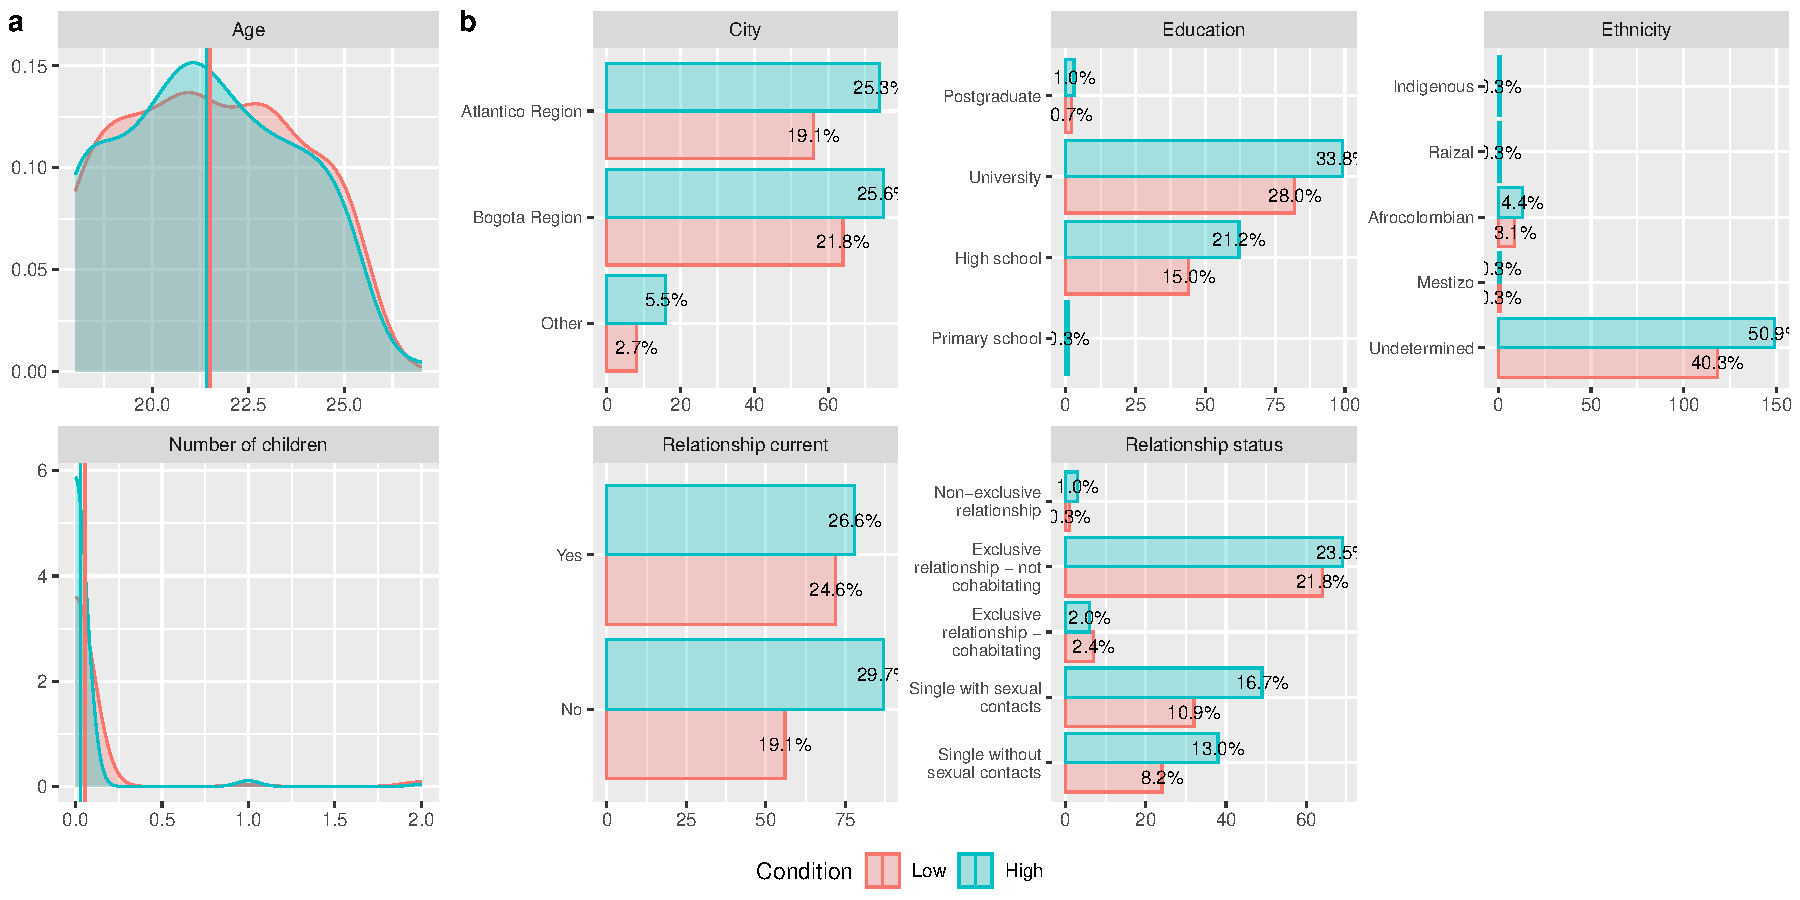
\includegraphics{Supplementary_material_files/figure-latex/sociodemographic-factors-desc-plot-1.pdf}
\caption{\label{fig:sociodemographic-factors-desc-plot}Distribution of values across sociodemographic variables, by condition.\textbf{a.} Distribution of values across numeric sociodemographic variables. Colored vertical lines indicate the mean value for each variable under each condition. \textbf{b.} Proportional number of participants across categorical variables.}
\end{figure}

\subsection{Access to resources}\label{access-to-resources}

\begin{Shaded}
\begin{Highlighting}[]
\CommentTok{\# Create a plot that displays the distribution of socioeconomic factors}
\CommentTok{\# by condition.}
\FunctionTok{ggarrange}\NormalTok{(}
  \CommentTok{\# Select relevant variables from the dataset (desc\_quest)}
\NormalTok{  desc\_quest }\SpecialCharTok{|\textgreater{}} 
  \FunctionTok{select}\NormalTok{(ID, Condition,}
\NormalTok{         Socioeconomic\_level, Electricity, Internet\_access, Internet\_use,}
\NormalTok{         TV, Hospital\_access) }\SpecialCharTok{|\textgreater{}}
  \CommentTok{\# Convert data from long to wide format to prepare for plotting}
  \FunctionTok{pivot\_longer}\NormalTok{(Socioeconomic\_level}\SpecialCharTok{:}\NormalTok{Hospital\_access,}
                \AttributeTok{names\_to =} \StringTok{"Variable"}\NormalTok{,}
                \AttributeTok{values\_to =} \StringTok{"Value"}\NormalTok{) }\SpecialCharTok{|\textgreater{}} 
  \CommentTok{\# Clean and transform the variable names by replacing underscores with spaces}
  \FunctionTok{mutate}\NormalTok{(}\AttributeTok{Variable =} \FunctionTok{str\_replace\_all}\NormalTok{(Variable, }\StringTok{"\_"}\NormalTok{, }\StringTok{" "}\NormalTok{)) }\SpecialCharTok{|\textgreater{}}
  \CommentTok{\# Create a plot of bar charts for socioeconomic variables, }
  \CommentTok{\# colored and filled by condition}
  \FunctionTok{ggplot}\NormalTok{(}\FunctionTok{aes}\NormalTok{(}\AttributeTok{y =}\NormalTok{ Value, }\AttributeTok{fill =}\NormalTok{ Condition, }\AttributeTok{color =}\NormalTok{ Condition)) }\SpecialCharTok{+}
  \FunctionTok{geom\_bar}\NormalTok{(}\AttributeTok{alpha =} \FloatTok{0.3}\NormalTok{, }\AttributeTok{position =} \FunctionTok{position\_dodge}\NormalTok{()) }\SpecialCharTok{+}  \CommentTok{\# Use semi{-}transparent bars}
  \CommentTok{\# Add text labels to display proportional values as percentages}
  \FunctionTok{geom\_text}\NormalTok{(}\FunctionTok{aes}\NormalTok{(}\AttributeTok{label =}\NormalTok{ scales}\SpecialCharTok{::}\FunctionTok{percent}\NormalTok{(}\FunctionTok{after\_stat}\NormalTok{(prop), }\AttributeTok{accuracy =} \FloatTok{0.1}\NormalTok{)),}
               \AttributeTok{xjust =} \StringTok{"inward"}\NormalTok{,}
               \AttributeTok{position =} \FunctionTok{position\_dodge}\NormalTok{(.}\DecValTok{9}\NormalTok{),}
               \AttributeTok{stat =} \StringTok{"prop"}\NormalTok{,}
               \AttributeTok{color =} \StringTok{"black"}\NormalTok{,}
               \AttributeTok{size =} \DecValTok{3}\NormalTok{) }\SpecialCharTok{+}
  \FunctionTok{facet\_wrap}\NormalTok{(}\SpecialCharTok{\textasciitilde{}}\NormalTok{Variable, }\AttributeTok{scales =} \StringTok{"free"}\NormalTok{) }\SpecialCharTok{+}  \CommentTok{\# Display variables in separate panels}
  \FunctionTok{scale\_y\_discrete}\NormalTok{(}\AttributeTok{labels =} \FunctionTok{label\_wrap}\NormalTok{(}\DecValTok{20}\NormalTok{)) }\SpecialCharTok{+}  \CommentTok{\# Wrap long labels for categorical axes}
  \FunctionTok{theme}\NormalTok{(}\AttributeTok{axis.text.y =} \FunctionTok{element\_text}\NormalTok{(}\AttributeTok{size =} \DecValTok{8}\NormalTok{)) }\SpecialCharTok{+}  \CommentTok{\# Reduce font size for y{-}axis text}
  \FunctionTok{labs}\NormalTok{(}\AttributeTok{x =} \ConstantTok{NULL}\NormalTok{, }\AttributeTok{y =} \ConstantTok{NULL}\NormalTok{),  }\CommentTok{\# Remove axis labels}
  \CommentTok{\# Arrange subplots into a grid with specified widths and share legends}
  \AttributeTok{widths =} \FunctionTok{c}\NormalTok{(}\DecValTok{1}\NormalTok{, }\DecValTok{3}\NormalTok{),}
  \AttributeTok{common.legend =} \ConstantTok{TRUE}\NormalTok{,}
  \AttributeTok{legend =} \StringTok{"bottom"}
\NormalTok{)}
\end{Highlighting}
\end{Shaded}

\begin{figure}
\centering
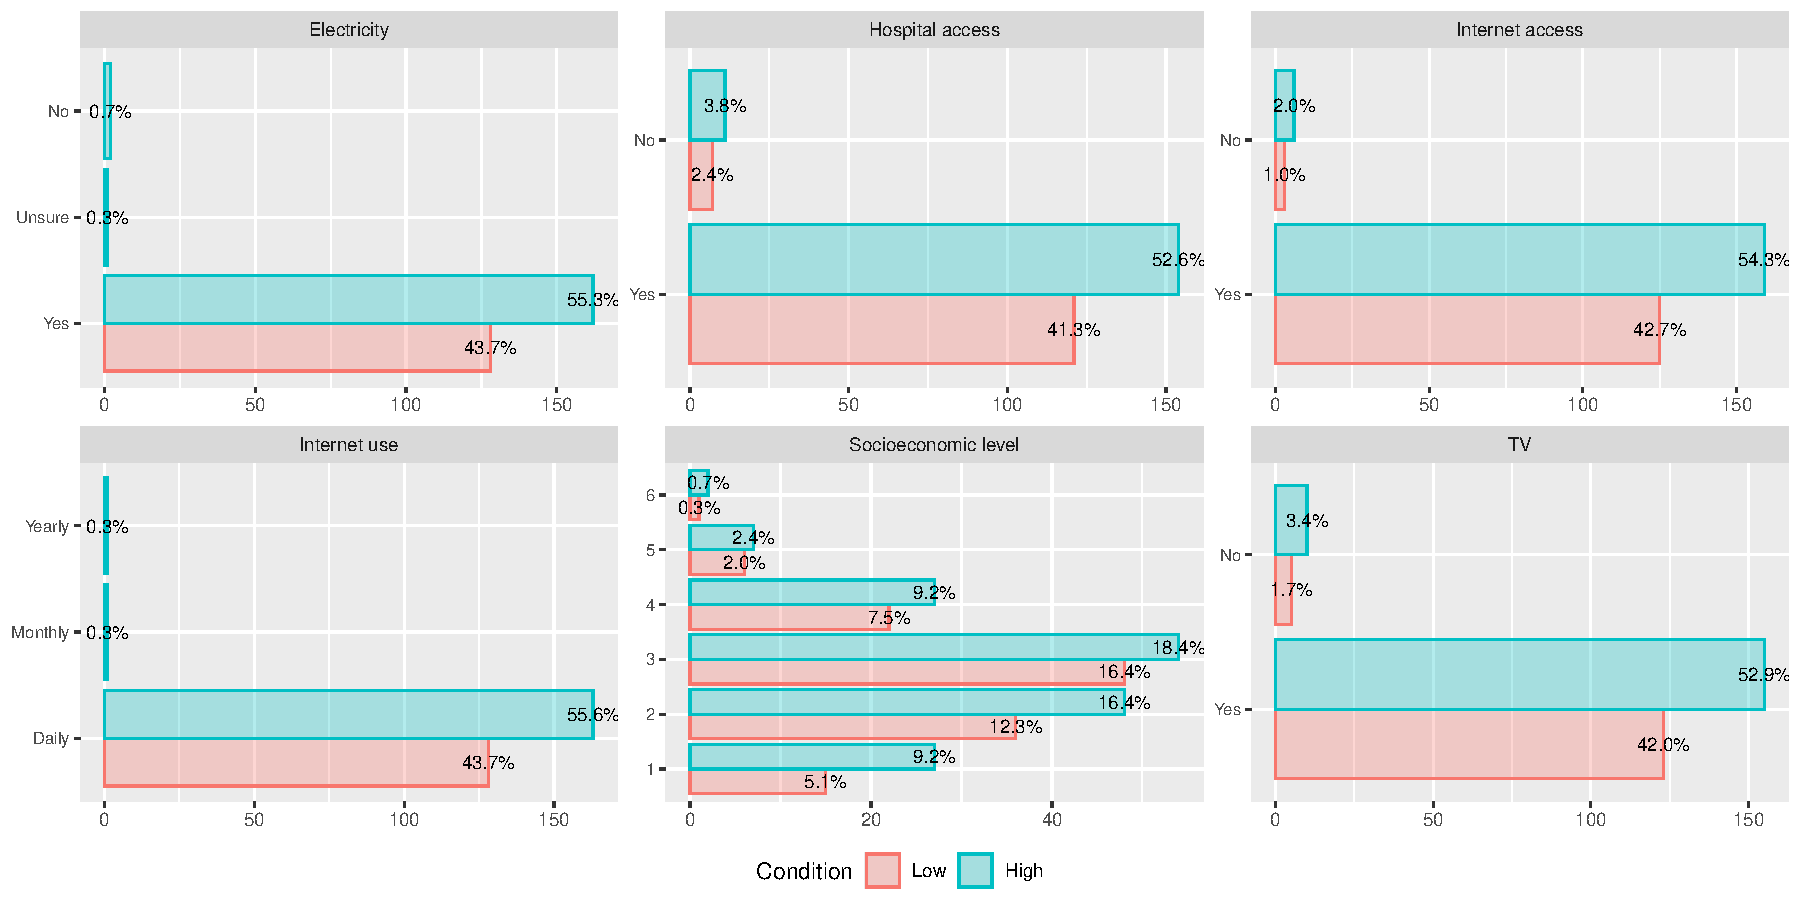
\includegraphics{Supplementary_material_files/figure-latex/resource-desc-plot-1.pdf}
\caption{\label{fig:resource-desc-plot}Proportional number of participants across categorical variables that measure access to resources.}
\end{figure}

\section{Session info (for reproducibility)}\label{session}

\begin{Shaded}
\begin{Highlighting}[]
\FunctionTok{library}\NormalTok{(pander)}
\FunctionTok{pander}\NormalTok{(}\FunctionTok{sessionInfo}\NormalTok{(), }\AttributeTok{locale =} \ConstantTok{FALSE}\NormalTok{)}
\end{Highlighting}
\end{Shaded}

\textbf{R version 4.4.1 (2024-06-14)}

\textbf{Platform:} x86\_64-pc-linux-gnu

\textbf{attached base packages:}
\emph{stats4}, \emph{stats}, \emph{graphics}, \emph{grDevices}, \emph{utils}, \emph{datasets}, \emph{methods} and \emph{base}

\textbf{other attached packages:}
\emph{pander(v.0.6.5)}, \emph{effectsize(v.0.8.9)}, \emph{bbmle(v.1.0.25.1)}, \emph{gtools(v.3.9.5)}, \emph{FactoMineR(v.2.11)}, \emph{factoextra(v.1.0.7)}, \emph{scales(v.1.3.0)}, \emph{GGally(v.2.2.1)}, \emph{performance(v.0.12.2)}, \emph{kableExtra(v.1.4.0)}, \emph{emmeans(v.1.10.3)}, \emph{lmerTest(v.3.1-3)}, \emph{lme4(v.1.1-35.5)}, \emph{Matrix(v.1.7-0)}, \emph{readxl(v.1.4.3)}, \emph{ggpubr(v.0.6.0)}, \emph{lubridate(v.1.9.3)}, \emph{forcats(v.1.0.0)}, \emph{stringr(v.1.5.1)}, \emph{dplyr(v.1.1.4)}, \emph{purrr(v.1.0.2)}, \emph{readr(v.2.1.5)}, \emph{tidyr(v.1.3.1)}, \emph{tibble(v.3.2.1)}, \emph{ggplot2(v.3.5.1)}, \emph{tidyverse(v.2.0.0)}, \emph{ggstats(v.0.6.0)}, \emph{MASS(v.7.3-61)}, \emph{car(v.3.1-2)}, \emph{carData(v.3.0-5)} and \emph{knitr(v.1.48)}

\textbf{loaded via a namespace (and not attached):}
\emph{gridExtra(v.2.3)}, \emph{rlang(v.1.1.4)}, \emph{magrittr(v.2.0.3)}, \emph{compiler(v.4.4.1)}, \emph{systemfonts(v.1.1.0)}, \emph{vctrs(v.0.6.5)}, \emph{pkgconfig(v.2.0.3)}, \emph{fastmap(v.1.2.0)}, \emph{backports(v.1.5.0)}, \emph{labeling(v.0.4.3)}, \emph{utf8(v.1.2.4)}, \emph{rmarkdown(v.2.28)}, \emph{tzdb(v.0.4.0)}, \emph{nloptr(v.2.1.1)}, \emph{xfun(v.0.47)}, \emph{flashClust(v.1.01-2)}, \emph{highr(v.0.11)}, \emph{broom(v.1.0.6)}, \emph{cluster(v.2.1.6)}, \emph{R6(v.2.5.1)}, \emph{stringi(v.1.8.4)}, \emph{RColorBrewer(v.1.1-3)}, \emph{boot(v.1.3-30)}, \emph{cellranger(v.1.1.0)}, \emph{numDeriv(v.2016.8-1.1)}, \emph{estimability(v.1.5.1)}, \emph{Rcpp(v.1.0.13)}, \emph{bookdown(v.0.40)}, \emph{parameters(v.0.22.1)}, \emph{splines(v.4.4.1)}, \emph{timechange(v.0.3.0)}, \emph{tidyselect(v.1.2.1)}, \emph{rstudioapi(v.0.16.0)}, \emph{abind(v.1.4-5)}, \emph{yaml(v.2.3.10)}, \emph{lattice(v.0.22-5)}, \emph{plyr(v.1.8.9)}, \emph{withr(v.3.0.1)}, \emph{bayestestR(v.0.14.0)}, \emph{coda(v.0.19-4.1)}, \emph{evaluate(v.0.24.0)}, \emph{xml2(v.1.3.6)}, \emph{pillar(v.1.9.0)}, \emph{DT(v.0.33)}, \emph{insight(v.0.20.2)}, \emph{generics(v.0.1.3)}, \emph{hms(v.1.1.3)}, \emph{munsell(v.0.5.1)}, \emph{minqa(v.1.2.7)}, \emph{xtable(v.1.8-4)}, \emph{leaps(v.3.2)}, \emph{glue(v.1.7.0)}, \emph{scatterplot3d(v.0.3-44)}, \emph{tools(v.4.4.1)}, \emph{ggsignif(v.0.6.4)}, \emph{mvtnorm(v.1.2-5)}, \emph{cowplot(v.1.1.3)}, \emph{grid(v.4.4.1)}, \emph{bdsmatrix(v.1.3-7)}, \emph{datawizard(v.0.12.2)}, \emph{colorspace(v.2.1-1)}, \emph{nlme(v.3.1-165)}, \emph{cli(v.3.6.3)}, \emph{fansi(v.1.0.6)}, \emph{viridisLite(v.0.4.2)}, \emph{svglite(v.2.1.3)}, \emph{gtable(v.0.3.5)}, \emph{rstatix(v.0.7.2)}, \emph{digest(v.0.6.37)}, \emph{ggrepel(v.0.9.5)}, \emph{htmlwidgets(v.1.6.4)}, \emph{farver(v.2.1.2)}, \emph{htmltools(v.0.5.8.1)}, \emph{lifecycle(v.1.0.4)} and \emph{multcompView(v.0.1-10)}

\section{Supplementary references}\label{refs}

\begin{multicols}{2}
\AtNextBibliography{\footnotesize}
\printbibliography[heading=none]
\normalsize
\end{multicols}

\def\printbibliography{}

\printbibliography

\end{document}
